
\documentclass[12pt, a4paper]{article}
\usepackage{ragged2e}
\usepackage[margin=1in]{geometry}
\usepackage[utf8]{inputenc}
\usepackage[capposition=top]{floatrow}
%\usepackage[tablesfirst,nolists]{endfloat}
\usepackage{times}
\usepackage[flushleft]{threeparttable}
\usepackage{hyperref}
\usepackage{authblk}
\usepackage{setspace}
\usepackage{apacite}
\usepackage{url}
\usepackage{caption}
\usepackage{graphicx}
\usepackage{titlesec}
\usepackage{color}
\usepackage{endnotes}
\usepackage{caption}
\usepackage{textcase}
\usepackage{booktabs}
\usepackage{titling}
\usepackage{rotating}
\usepackage{amsmath}
\usepackage{bm}
\usepackage{authblk}
\usepackage{adjustbox}
\usepackage[section]{placeins}
\usepackage[toc,page]{appendix}
\usepackage{parskip}

\newcommand{\AT}[1]{\textcolor{red}{AT: #1}}
\newcommand{\NS}[1]{\textcolor{green}{NS: #1}}
\newcommand{\TM}[1]{\textcolor{blue}{TM: #1}}

% Keywords command
\providecommand{\keywords}[1]
{
  \small	
  \textbf{\textit{Keywords---}} #1
}

\captionsetup{
  labelsep=newline,
  justification=raggedright,
  singlelinecheck=false
}

\pagestyle{myheadings}
\title{}
\author{}
\date{}
\doublespacing
%\renewcommand{\efloatheading}[1]{}


\titleformat{name=\section,numberless}[hang]
   {\bfseries}{}{6pt}{\Large}


\let\footnote=\endnote
\newcommand{\vect}[1]{\boldsymbol{#1}}

\bibliographystyle{apacite}
\begin{document}

\title{The role of alcohol in the link between national football tournaments (soccer) and domestic abuse - evidence from England}

\author{Anna Trendl$^{a,*}$ \\ \href{mailto:a.trendl@warwick.ac.uk}{a.trendl@warwick.ac.uk}\\
 \and Neil Stewart$^a$ \\ 
 \href{mailto:neil.stewart@wbs.ac.uk}{Neil.Stewart@wbs.ac.uk}
 \\ 
 \and Timothy L. Mullett$^a$ \\
 \href{mailto:Tim.Mullett@wbs.ac.uk}{Tim.Mullett@wbs.ac.uk}
 \\}
 
\date{
    $^a$Warwick Business School, University of Warwick, Scarman Road, Coventry, CV4 7AL, UK\\
    $^*$Corresponding author\\[2ex]%
    \today
}



\begin{titlepage}


\maketitle
\thispagestyle{empty}
\centering
This research was funded in part by Economic and Social Research Council grants ES/K002201/1, ES/P008976/1, and ES/N018192/1, and Leverhulme Trust grant RP2012-V-022. 
\clearpage
\thispagestyle{empty}
\RaggedRight
%\begin{center}
%\LARGE{The link between national football tournaments and alcohol-related domestic abuse - evidence from England}
%\end{center}
%\begin{abstract}
%\noindent

\begin{abstract}
\noindent


Domestic abuse is increasingly recognised as a serious public health concern worldwide. Previous research has suggested a link between national football (soccer) tournaments and domestic abuse. While hypothesized to be a significant factor, the role alcohol plays in this relationship has not yet been explored quantitatively. In this study, using 10 years' worth of crime data (from 2010 to 2019) from the third largest police force in England (West Midlands police), we explored the effect of England draws, losses, and wins in national football tournaments on the number of alcohol and non-alcohol-related domestic abuse cases reported to the police. Results from a series of negative binomial regression analyses show that the number of reported alcohol-related domestic abuse cases increases by 47\%, 95\% confidence interval [26\% -- 71\%], following an England football victory. This effect is limited to alcohol-related cases. The estimate translates into a 0.53, 95\% CI [0.3 -- 0.8], increase in the daily rate of alcohol-related cases per 100,000 individuals. The England win effect survives various robustness checks (including the re-analysis of a dataset from another geographical area in England), and its time course is strongly consistent with a causal link between England's football victories and an increase in alcohol-related domestic abuse. We also found a comparable increase in the number of other (non-domestic abuse related) alcohol-related violent crimes on England win days. Further research is required to understand the exact causal pathway between national football tournaments, alcohol consumption, and violent behaviours in domestic settings.




\end{abstract}

\keywords{football, domestic abuse, alcohol}

\end{titlepage}



\newpage
\RaggedRight
\section{Introduction}


Domestic abuse is considered to be a major public policy concern in many countries, including the UK \cite{ep}. While anyone can become a victim of domestic abuse, women are disproportionately affected: an estimated 7.5\% of women and 3.8\% of men in England and Wales reported to have experienced some form of domestic abuse in the year ending March, 2019 \cite{ONS2019}.


The link between sporting events and domestic abuse has been the focus of a number of smaller studies \cite{Williams2014}, but large-scale quantitative investigations of this relationship are relatively scarce. In the context of the USA, the most extensive study in the topic found that an unexpected loss of the local National Football League (NFL) team resulted in a 10\% increase in the rate of reported male to female intimate partner violence (IPV; \citeNP{Card2011}.

In England, previous studies have focused on the link between football (soccer) and domestic abuse. Football's history is inextricably linked to England, and it is by far the most popular sport in the country \cite{Parry2014}, with the 2018 World Cup attracting a record number of 44.5 million viewers \cite{BBC}. These studies have found significant increases in the number of domestic abuse cases recorded by the police on England win, and particularly on England loss days \cite{Brimicombe2012, Kirby2014}. While domestic abuse is predominantly understood as a pattern of ongoing behaviour involving a series of occurrences, rather than a one-off incident triggered by football \cite{Brooks-Hay2018}, these studies, and other qualitative investigations (e.g., \citeNP{Swallow}) nevertheless suggest that national football tournaments can create an environment where domestic abuse is more likely to occur.




Why would national football tournaments, such as the World Cup or the European Championship precipitate domestic abuse? England's participation in these tournaments are times of heightened patriotic emotions and a strengthened sense of ``Englishness'', fuelled by media narratives that often use war references, and an ``us vs. them'' rhetoric to generate and represent an English national identity \cite{Vincent2014}. Previous qualitative research has suggested that televised contact sports can serve as vehicle for the male sports fan to redefine, and express his masculinity in a way that allows dominance, control, and can ultimately manifest in the perpetration of domestic abuse \cite{Sabo,Swallow}, given susceptibility to such behaviours. We speculate that this observation is especially pertinent in the context of England's participation in national football tournaments, owing to the popularity of the sport in the country, the associated media attention, and the resulting heightened sense of national consciousness. 

In England, televised coverages of national football tournaments are often sponsored by major alcohol brands. An analysis of the 2016 UEFA EURO broadcasts in the UK found that viewers encountered 122 references to alcohol per broadcast on average (0.65 per minute; \citeNP{Purves2017}). The strong association between sports spectatorship and alcohol consumption has been documented across various sports, including football (soccer; \citeNP{Durbeej2017a};\citeNP{Elgan2018}, \citeNP{Pearson2011}), American football \cite{Glassman2011}, and baseball \cite{Erickson2011}. In the context of English football culture, research has mostly focused on the role of alcohol in crowd violence (football hooliganism; e.g., \citeNP{Pearson2011};\citeNP{Cleland2016};\citeNP{Ostrowsky2014a}). 

Previous studies found a strong, but complex link between alcohol and domestic abuse, suggesting that alcohol can either be seen as a contributing cause, an aggravating factor, or a trigger of violent behaviour in domestic (and other) settings \cite{Leonard2017}. The ecological model of intimate partner violence (IPV; the most common form of domestic abuse) sees IPV as a product of societal, community, relationship, and individual influences. From a community perspective, \citeA{Graham2017} argue that social contexts where excessive drinking is encouraged (e.g., through the promotion of alcohol during sporting events) are often permissive of violent behaviour and sexism, which can increase the likelihood of alcohol-related domestic abuse. However, strong inhibitory factors (e.g., social norms, and more specifically the condemnation of peers) can offset the disinhibitory effect of alcohol consumption, and reduce the likelihood of subsequent perpetration.  



Despite the evident links between alcohol and domestic abuse, the role alcohol plays in the link between football and domestic abuse has not yet been explored in a large-scale quantitative study. Given the strong association between drinking culture and football in England \cite{Dixon2014}, a relationship continuously reinforced by the marketing practices of the alcohol industry \cite{Gornall2014}, we conjecture that alcohol acts as an aggravating factor in the link between football and domestic abuse in England. 

Specifically, we hypothesize that when the England national football team plays, the number of reported alcohol-related domestic abuse cases increases. Based on previous research focusing on the link between the football World Cup and domestic abuse in England (e.g., \citeNP{Brimicombe2012, Kirby2014}), we expect the effect to be stronger on England loss and win days. Exploring the link between football, alcohol, and domestic abuse will deepen our understanding of the pathway through which football (and more specifically the outcome of the match) increases propensity for violence in domestic settings.

In our analysis, we focus on the two largest national football tournaments England participates in, the the FIFA World Cup and UEFA European Football Championship. We exploit the fact that that national teams are randomly allocated (by the random draw of balls from an urn --- the canonical definition of random) to slots in these football tournaments, and the dates of these slots are assigned \emph{before} the allocation of the teams. This allows us to make causal claims about the effect of England matches on alcohol and non-alcohol related domestic abuse. In contrast, \citeA{Card2011} had to rely upon the stochastic nature of game outcomes (after controlling for bookmakers' expectations) to make a causal inference between unexpected losses NFL football and domestic abuse. 

To test our hypothesis, we investigate whether the daily number of reported alcohol and non-alcohol related domestic abuse cases recorded by the second largest police force in England (West Midlands Police; WMP) between 2010 and 2019 increase on days when the England national team plays in a national football tournament (the FIFA World Cup and UEFA European Football Championship), and whether the effect, if any, depends on the result of the match. Our dataset covers a decade, allowing us to conduct a thorough investigation of the characteristics and temporal pattern of the domestic abuse perpetrated on England match days, and extend our findings to understand various characteristics of this relationship. We also test the robustness of the effect using various model specifications, time periods, and geographical areas. 



\section{Datasets}

\subsection{West Midlands Crime Dataset}


Our dataset comprises all incidents and crimes recorded by the West Midlands Police (WMP) in the period between January 1, 2010 and October 10, 2019 (3570 days). The WMP is the third largest police force in England \cite{Homeoffice}, serving an area with a population over 2.9 million in 2018 \cite{populationfigure}. 

The WMP records all reported cases in two databases: incidents and crimes. The incidents database records all reports from officers and the public to call centres and police stations. The crimes database includes all cases which, after initial investigation, are found to meet the definition of a notifiable offence \citeNP{HomeOffice2019}, or fall into one of the special categories of ``non-crime''. These special categories include rape, domestic abuse, child abuse, racially or religiously aggravated cases, and are recorded in the crimes database (e.g., as ``domestic violence incident - non crime''), even if the investigation finds that they do not qualify as a notifiable offence (e.g., due to lack of evidence).
 
We focus our analyses on the crimes database, as these cases have been investigated by police. These records therefore contain more data and are more robust and reliable than incident logs. Officers record the age, gender and ethnicity for both victim and offender (note that the victim offender roles are judged and defined by the recording officer), as well as the location and exact time of the crime. 
In identifying which crimes constitute domestic abuse, we include all crime records for specific domestic abuse crimes and non-crimes. There are also a number of crimes which are recorded as non-domestic abuse offences, but which are, or result from domestic abuse (e.g., grievous bodily harm). To ensure we identify such cases, we link the records in the crimes database to that of the incidents data. The incidents database contains flags for a number of properties of the incidents \citeNP{HomeOffice2011}, including ``domestic abuse'' and ``alcohol''. Thus, any non-domestic abuse crimes were identified as domestic abuse if they also had such a domestic abuse flag in a linked incident record. Table \ref{crimetypes} In the Appendix lists the number and percentage of domestic abuse cases in the sample by offence code.

When identifying whether alcohol was involved, we primarily rely upon the specific alcohol flag in the crime record. When an officer records a crime, they must select any flags that are relevant to the case and one of these is ``alcohol involvement''. The definition for this is prescribed by the UK Home Office ``any notifiable offence (crime) where it is perceived, by the victim or any other person, that the effects of alcohol consumption on the offender or victim was an aggravating factor'' \cite{Office2019}. Note that this definition applies to the incident in general, not to either the offender or victim specifically. Since this flag must be actively selected by the recording officer, there is a potential for under reporting. To ameliorate this, we again relied on the flags in the incidents data, and also examined the free text records of the associated incident log. If any linked incident record contained a reference to alcohol (either in the free text or as a flag) then it was also identified as alcohol related.


 Overall there were 427,351 reported cases of domestic abuse in this 10-year period, comprising 17\% of all recorded crimes and incidents. Of these cases, 26\% were alcohol-related (in contrast, only 9\% of non domestic abuse cases are alcohol-related). However, it is worth noting that the identification of alcohol-involvement is likely to be more precise for domestic abuse cases, where the victim and offender know each other, as opposed to other types of criminal behaviours (especially where the offender is unknown). In the period between 2010 and 2018, the daily rate of non-alcohol related domestic incidents is between 1.42--3.95 cases per 100,000 individuals, whereas the daily rate of alcohol-related cases is between 0.84--1.67 cases per 100,000 individuals (the overall rate is between 2.40--5.01 per 100,000 individuals). 
 

Figure \ref{fig:descriptive} shows the daily average number of alcohol and non-alcohol related domestic abuse cases reported to WMP by day of the week. The reported number of domestic abuse cases, and particularly alcohol-related cases shows strong variation throughout the week, with generally fewer reported cases mid-week, and a pronounced increase over the weekend. 

\begin{figure} 
\begin{center} 
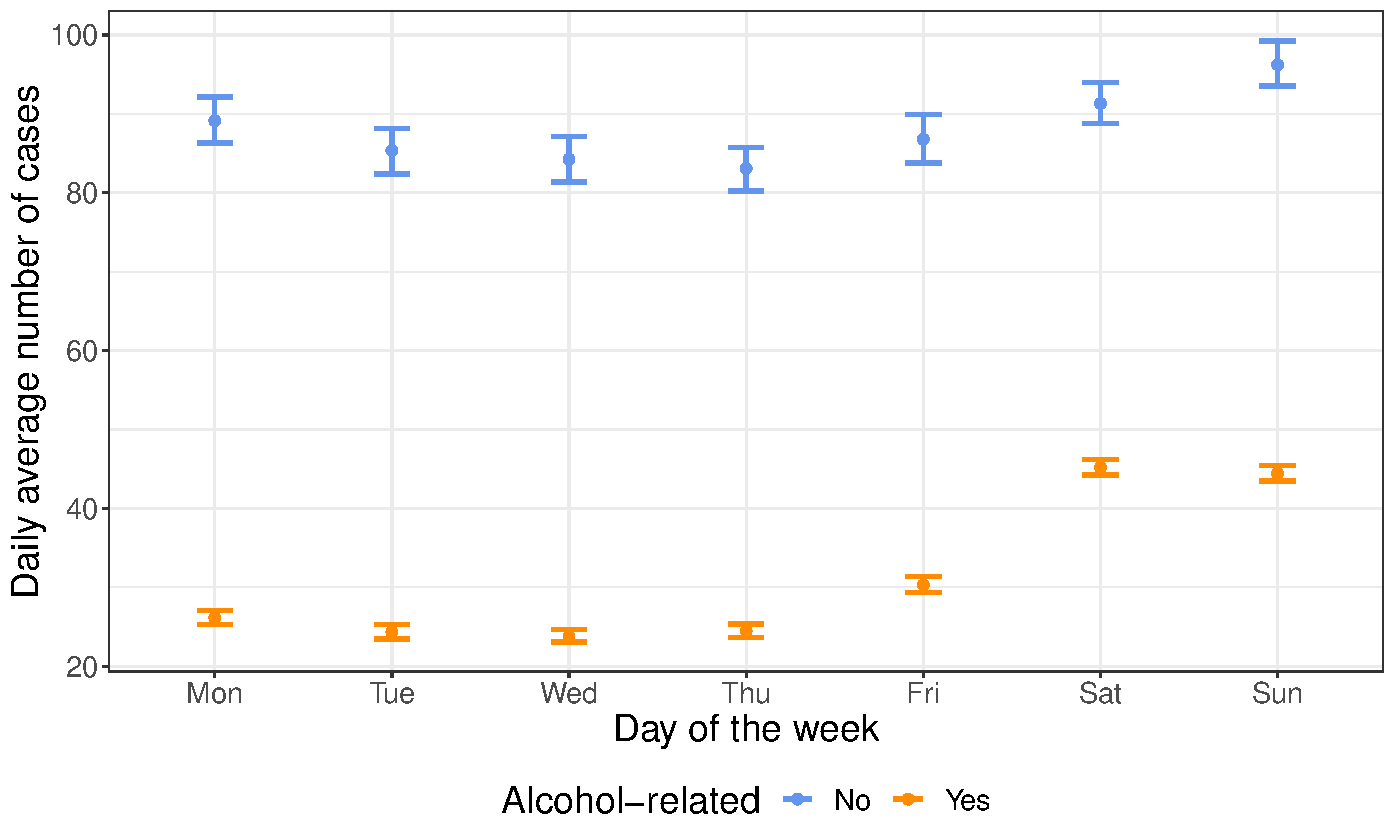
\includegraphics[scale = 0.6]{descriptives.pdf}
\caption{The daily average number of alcohol and non-alcohol related domestic abuse cases reported to the police, by day of the week. The error bars show bootstrapped 95\% confidence intervals, stratified by month. \label{fig:descriptive}} 
\end{center} 
\end{figure} 

In the UK, the term ``domestic abuse'' refers to a wide range of behavioural patterns, from physical and sexual violence to psychological, emotional, financial abuse, threatening behaviour, stalking and harassment, either within a family or an intimate relationship \cite{ONS}. Previous research has mostly focused on intimate partner violence (IPV), the largest subcategory of domestic abuse. While IPV is more common than abuse perpetrated by family members \cite{ONS}, our dataset does not contain information about the exact relationship between the victim and perpetrator (family versus current or ex-partner), therefore we cannot separate the two types of abuse, and we will refer to them collectively as ``domestic abuse''.

In our analyses, we explore various characteristics of domestic abuse and other criminal behaviours (not classified as domestic abuse) perpetrated on England football days. Specifically, we focus on property-related crimes (where the offence class is either theft or robbery), hate crimes (where the offence description includes the words ``hate'', ``racial'' or ``racially''), and other violent crimes, where the offence class is classified as violence against the person, after excluding cases of domestic abuse. 

We also explore specific characteristics of domestic abuse cases. To this end, we classify domestic abuse cases by whether they are newly reported (with no earlier record for the same victim-offender pair in our dataset), publicly perpetrated (cases where the location is not a residential dwelling), or result in an injury (where the injury class is either minor or serious injury). In addition, we will examine how reporting behaviour (measured by the number of hours elapsed between time of perpetration and reporting), and in the case of repeat incidents (multiple cases with the same victim-offender pair), days elapsed between subsequent cases (days since last case, days until next case) are affected by England football matches.



Our dataset contains all cases of domestic abuse that have been reported to the WMP between 2010 and 2019, but the vast majority of domestic abuse incidents in fact never get reported (according to the Crime Survey of England and Wales, only 17\% of domestic abuse victims reported the abuse to the police between April 2017 and March 2018; \citeNP{ONS}). This substantial reporting bias, and its potential correlation with other contextual factors warrants a careful interpretation of the estimates from any quantitative study investigating domestic abuse, and highlights the importance of utilising a mixed methods approach to explore the factors contributing to the prevalence of domestic abuse. 
  
 \subsection{Sports data}
 
\begin{table}
\centering
    \caption{Matches of the England national football team in the World Cup and European Championship football tournaments between 2010 and 2019, by outcome.}
\begin{tabular}{ccccc}
  \hline
\textbf{Date} & \textbf{Other Team} & \textbf{Tournament} & \textbf{Year} & \textbf{Outcome} \\ 
  \hline
2010-06-12 & USA & World Cup & 2010 & England draw \\ 
  2010-06-18 & Algeria & World Cup & 2010 & England draw \\ 
  2010-06-23 & Slovenia & World Cup & 2010 & England win \\ 
  2010-06-27 & Germany & World Cup & 2010 & England lost \\ 
  2012-06-11 & France & European Championship & 2012 & England draw \\ 
  2012-06-15 & Sweden & European Championship & 2012 & England win \\ 
  2012-06-19 & Ukraine & European Championship & 2012 & England win \\ 
  2012-06-24 & Italy & European Championship & 2012 & England lost \\ 
  2014-06-14 & Italy & World Cup & 2014 & England lost \\ 
  2014-06-19 & Uruguay & World Cup & 2014 & England lost \\ 
  2014-06-24 & Costa Rica & World Cup & 2014 & England draw \\ 
  2016-06-11 & Russia & European Championship & 2016 & England draw \\ 
  2016-06-16 & Wales & European Championship & 2016 & England win \\ 
  2016-06-20 & Slovakia & European Championship & 2016 & England draw \\ 
  2016-06-27 & Iceland & European Championship & 2016 & England lost \\ 
  2018-06-18 & Tunisia & World Cup & 2018 & England win \\ 
  2018-06-24 & Panama & World Cup & 2018 & England win \\ 
  2018-06-28 & Belgium & World Cup & 2018 & England lost \\ 
  2018-07-03 & Colombia & World Cup & 2018 & England win \\ 
  2018-07-07 & Sweden & World Cup & 2018 & England win \\ 
  2018-07-11 & Croatia & World Cup & 2018 & England lost \\ 
  2018-07-14 & Belgium & World Cup & 2018 & England lost \\ 
   \hline
\end{tabular}
  \label{Tab:matches}
\end{table}

 There were three World Cups (2010, 2014, 2018) and two European Championships (2012, 2016) in the period covered by our dataset. All of these tournaments took place in the months of June and July. 
Table \ref{Tab:matches} shows the matches of the English national football team in these tournaments. Out of 22 matches overall, England won and lost both eight times, while six matches ended in a draw. 

While the main focus of this study is the effect of football on domestic abuse, to investigate whether the association between football and domestic abuse can be observed for other sports, we also focus on rugby, the second most popular sport in England \cite{Ipsos2003}. Specifically, we obtained historical results data from the Six Nations tournament, a high-profile international rugby tournament that takes place every year in the months of February and March with the participation of England, Wales, Scotland, Ireland, France and Italy. Each tournament year, England plays one match with each of the other five participating countries, and these matches take place almost always during the weekend (Saturday, $N = 37$; Sunday, $N = 11$; Friday, $N = 2$). The most common result for England is to win ($N = 35$), much less frequent are losses ($N = 12$), and draws ($N = 2$).

\section{Methods}


To investigate the role alcohol plays in the link between England football matches and domestic abuse, we used a regression framework. Our main results are derived from Poisson and Negative Binomial regressions, where each observation is a day or a three-hour interval in the period between 2010 and 2019, and the outcome variable is the number of cases perpetrated in an observation period. To investigate certain characteristics of the domestic abuse cases perpetrated on England match days, we also used a logistic regression framework. Below is a detailed explanation of the statistical models used in our analyses.  


\subsection{Count per day analyses} 
\label{modelsexplained}


In these regressions, each day in our dataset is an observation (of which there are 3570), and the outcome variable is the number of domestic abuse cases perpetrated on that day (alcohol-related or not). We classified each day in this period as one of the following: England won (England win, $N = 8$), lost (England lost, $N = 8$) or drew (England draw, $N = 6$), a day after an England match day (After England, $N = 22$), any other day during the months of the tournament (Tournament on, $N = 106$), or any other day during the rest of the year (Non-match day, $N = 3420$). Our aim is to understand the extent to which this classification variable can explain the number of alcohol-related and non-alcohol related cases reported to the police.

To control for potential confounders and account for the temporal variability of the number of domestic abuse cases, we also added a set of dummy  variables, including day of the week, calendar month, and year. 
We included a dummy for Christmas cases (covering the period between 24th and 26th of December) and New Year's Eve cases (cases perpetrated on the 1st of January). 
These holidays are consistently associated with an increased number of domestic abuse cases reported to the police, therefore including these will result in a more precise estimate of the association between football and domestic abuse.

Given that our outcome variable is a count, we considered using a Poisson or a negative binomial regression model framework. 
Formally, if $C_i$ is the number of reported cases (alcohol or non-alcohol related) on days $i = 1...N$, then these models can be formally expressed as
%
\begin{equation}
 \ln(\lambda_i) =\vect{x_i^{T}}\vect{\beta}
\end{equation}


where 
$C_i \sim Pois(\lambda_i)$ or $C_i \sim Negative Binomial(\lambda_i,\theta)$, $\vect{x_i}$, is a vector of covariates, and $\boldsymbol{\beta}$ is the vector of coefficients.

In the Poisson framework, it is assumed that the mean of the distribution ($\lambda_i$) is equal to the variance. 
However, for certain types of count data, the observed variance can exceed the mean, causing overdispersion. 
If overdispersion is present in the data, the Poisson model understates the standard error of the estimates, leading to erroneous conclusions. 
Given the complex nature of domestic abuse, it is likely that our model will not able to fully account for all the factors influencing the number of reported cases on a given day, leading to unobserved heterogeneity and increasing the likelihood of overdispersion. 
Testing for overdispersion in a Poisson model involves testing the null-hypothesis of equidispersion (the mean being equal to the variance).
If there is evidence for overdispersion, a negative binomial model is a more suitable modelling framework, as it includes an additional parameter $\theta$ to allow the variance to deviate from the mean. 


\subsection{Count per three-hour interval analysis}

In this analysis, we used the regression framework described in section \ref{modelsexplained} (either Poisson or negative binomial regression) to investigate the temporal dynamics of the number of domestic abuse cases (alcohol-related or not) perpetrated before and after England matches. To this end, we divided each day in our dataset into eight three-hour periods, the first one starting at 12am, and used these to identify specific time windows around the time of the match (six and three hours before the match, during match, and three, six, twelve, and twenty-four hours after the match). The exact time of the matches vary considerably (the earliest starting at 1pm, and the latest at 11pm). We first identified the three-hour period of the day into which each match falls. If the start and end time of the match did not fall in the same three-hour period, we chose the three-hour period that covers the larger part of the match (e.g., a 2.5 hour long match starting at 7pm will be assigned to the 6-9pm period and not to the 9pm-12am period). In these regressions, each time window indicator is a dummy variable, therefore the exponentiated coefficients directly represent the relative change in the number of cases during these periods, compared to any other (overwhelmingly non-match) periods. To control for potential confounders, we controlled for year, month, day of week, three-hour period of the day, Christmas and New Year's Eve.


\subsection{Binary outcome variable analyses}

To further understand the characteristics of domestic abuse cases perpetrated on England football days, such as whether these cases are more likely to occur in a public location or end in serious injury, we used a logistic regression framework. 
Given a binary response variable ($Y_{i}$ can either take the value 0 or 1), we wish to model the probability of an event occurring, i.e., $\pi = P(Y = 1)$. 
In a logistic regression framework, we can model this probability with the equation

\begin{equation}
log(\frac{\pi}{1-\pi})= \vect{x_i^{T}}\vect{\beta}
\end{equation}

where \textbf{x\textsubscript{i}} is a vector of covariates, and $\boldsymbol{\beta}$ is the vector of coefficients.


\newpage

\section{Results}

In the following count per day analyses (sections \ref{firstsection}--\ref{lastsection}), the results are almost exclusively derived from negative binomial models (unless noted otherwise), as we found evidence for overdispersion in almost all cases (after testing for overdispersion using the method described in \citeNP{Cameron1990a}). All analyses were performed in R (version 3.6.2).


\subsection{Core results} \label{firstsection}

Table \ref{coremodel} shows the results from two negative binomial regressions investigating the link between football, alcohol and domestic abuse. The first column shows the results for the subset of non-alcohol-related cases, while the second column shows the estimates for alcohol-related cases. For non-alcohol-related cases, we find no evidence for an increase (or decrease) on days when the England football team plays, compared to non-match days. In contrast, we see a significant 47\% increase, 95\% CI [26\%--71\%], in the number of alcohol-related cases on days when the England football team wins, compared to non-match days. We find no evidence for comparable increases in the number of reported domestic abuse cases when the England national team loses or draws. In addition, we estimate that there is an 18\% increase, 95\% CI [7\%--30\%], in the number of alcohol-related cases reported after an England match day. 


%\begin{table*}[!htbp] \centering 
%  \begin{threeparttable}
%  \caption{The effect of England football days on domestic abuse by alcohol-involvement, 2010-2019} 
%  \label{coremodel} 
%\begin{tabular}{@{\extracolsep{5pt}}lcc} 
%\\[-1.8ex]\hline 
%\hline \\[-1.8ex] 
% & \multicolumn{2}{c}{\textit{Dependent variable:}} \\ 
%\cline{2-3} 
%\\[-1.8ex] & \multicolumn{2}{c}{Number of domestic abuse cases} \\ 
% & Non-alcohol-related & Alcohol-related\\ 
%\\[-1.8ex] & (1) & (2)\\ 
%%\hline \\[-1.8ex] 
%\hline \\[-1.8ex] 
% Tournament on & 1.024 & 0.984 \\ 
%  & [0.986, 1.064] & [0.935, 1.037] \\ 
%  & & \\ 
% England win & 0.950 & 1.469$^{***}$ \\ 
%  & [0.838, 1.077] & [1.259, 1.714] \\ 
%  & & \\ 
% England draw & 1.045 & 1.145 \\ 
%  & [0.905, 1.208] & [0.955, 1.375] \\ 
%  & & \\ 
% England lost & 1.033 & 1.129 \\ 
%  & [0.915, 1.167] & [0.963, 1.324] \\ 
%  & & \\ 
% After England  & 1.056 & 1.181$^{**}$ \\ 
%  & [0.979, 1.140] & [1.069, 1.305] \\ 
%\hline \\[-1.8ex] 
%Observations & 3,570 & 3,570 \\ 
%%Log Likelihood & $-$14,692.790 & $-$12,071.110 \\ 
%%$\theta$ & 51.259$^{***}$  (1.967) & 39.423$^{***}$  (2.112) \\ 
%%Akaike Inf. Crit. & 29,453.580 & 24,210.210 \\ 
%\hline 
%\hline \\[-1.8ex] 
%Notes:
%%\textit{Note:}  & \multicolumn{2}{r}{$^{*}$p$<$0.1; $^{**}$p$<$0.05; $^{***}$p$<$0.01} \\ 
%\end{tabular} 
%\begin{tablenotes}
%      \item[a] \textit{$^{*}$p$<$0.05; $^{**}$p$<$0.01; $^{***}$p$<$0.001}
%      \item[b] \textit{Estimates are exponentiated coefficients from negative binomial regressions with non-match day as benchmark; controls include day of week, month, year, Christmas, and New Year's Eve; 95\% confidence intervals are in square brackets}
%    \end{tablenotes}
%\end{threeparttable} 
%\end{table*}



\begin{table*}[!htbp] \centering 
  \begin{threeparttable}
  \caption{The effect of England football days on domestic abuse by alcohol-involvement, 2010-2019} 
  \label{coremodel} 
\begin{tabular}{@{\extracolsep{5pt}}lcc} 
\\[-1.8ex]\hline 
\hline \\[-1.8ex] 
 & \multicolumn{2}{c}{\textit{Dependent variable:}} \\ 
\cline{2-3} 
\\[-1.8ex] & \multicolumn{2}{c}{Number of domestic abuse cases} \\ 
 & Non-alcohol-related & Alcohol-related\\ 
\\[-1.8ex] & (1) & (2)\\ 
\hline \\[-1.8ex] 
 Tournament on & 1.024 & 0.984 \\ 
  & [0.986, 1.064] & [0.935, 1.037] \\ 
  & (0.218) & (0.552) \\ 
  & & \\ 
 England win & 0.950 & 1.469$^{*}$ \\ 
  & [0.838, 1.077] & [1.259, 1.714] \\ 
  & (0.423) & (0.00001) \\ 
  & & \\ 
 England draw & 1.045 & 1.145 \\ 
  & [0.905, 1.208] & [0.955, 1.375] \\ 
  & (0.551) & (0.146) \\ 
  & & \\ 
 England lost & 1.033 & 1.129 \\ 
  & [0.915, 1.167] & [0.963, 1.324] \\ 
  & (0.603) & (0.136) \\ 
  & & \\ 
 After England & 1.056 & 1.181$^{*}$ \\ 
  & [0.979, 1.140] & [1.069, 1.305] \\ 
  & (0.159) & (0.002) \\ 
  & & \\ 
\hline \\[-1.8ex] 
Observations & 3,570 & 3,570 \\ 
%Log Likelihood & $-$14,692.790 & $-$12,071.110 \\ 
%$\theta$ & 51.259$^{***}$  (1.967) & 39.423$^{***}$  (2.112) \\ 
%Akaike Inf. Crit. & 29,453.580 & 24,210.210 \\ 
\hline 
\hline \\[-1.8ex] 
%\textit{Note:}  & \multicolumn{2}{r}{$^{*}$p$<$0.05; $^{**}$p$<$0.01; $^{***}$p$<$0.001} \\ 
\end{tabular}  
\begin{tablenotes}
      \item[a] \textit{Estimates are exponentiated coefficients from negative binomial regressions with non-match day as benchmark; controls include day of week, month, year, Christmas, and New Year's Eve; 95\% confidence intervals are in square brackets, p-values are in parentheses}
       \item[b] \textit{Coefficients denoted with $*$ are significant at Bonferroni-corrected alpha levels}
    \end{tablenotes}
\end{threeparttable} 
\end{table*}




 \begin{figure}[!htbp]
\centering
 \caption{The temporal dynamics of the number of domestic abuse cases perpetrated on England draw, lose, and win days, by alcohol involvement.}
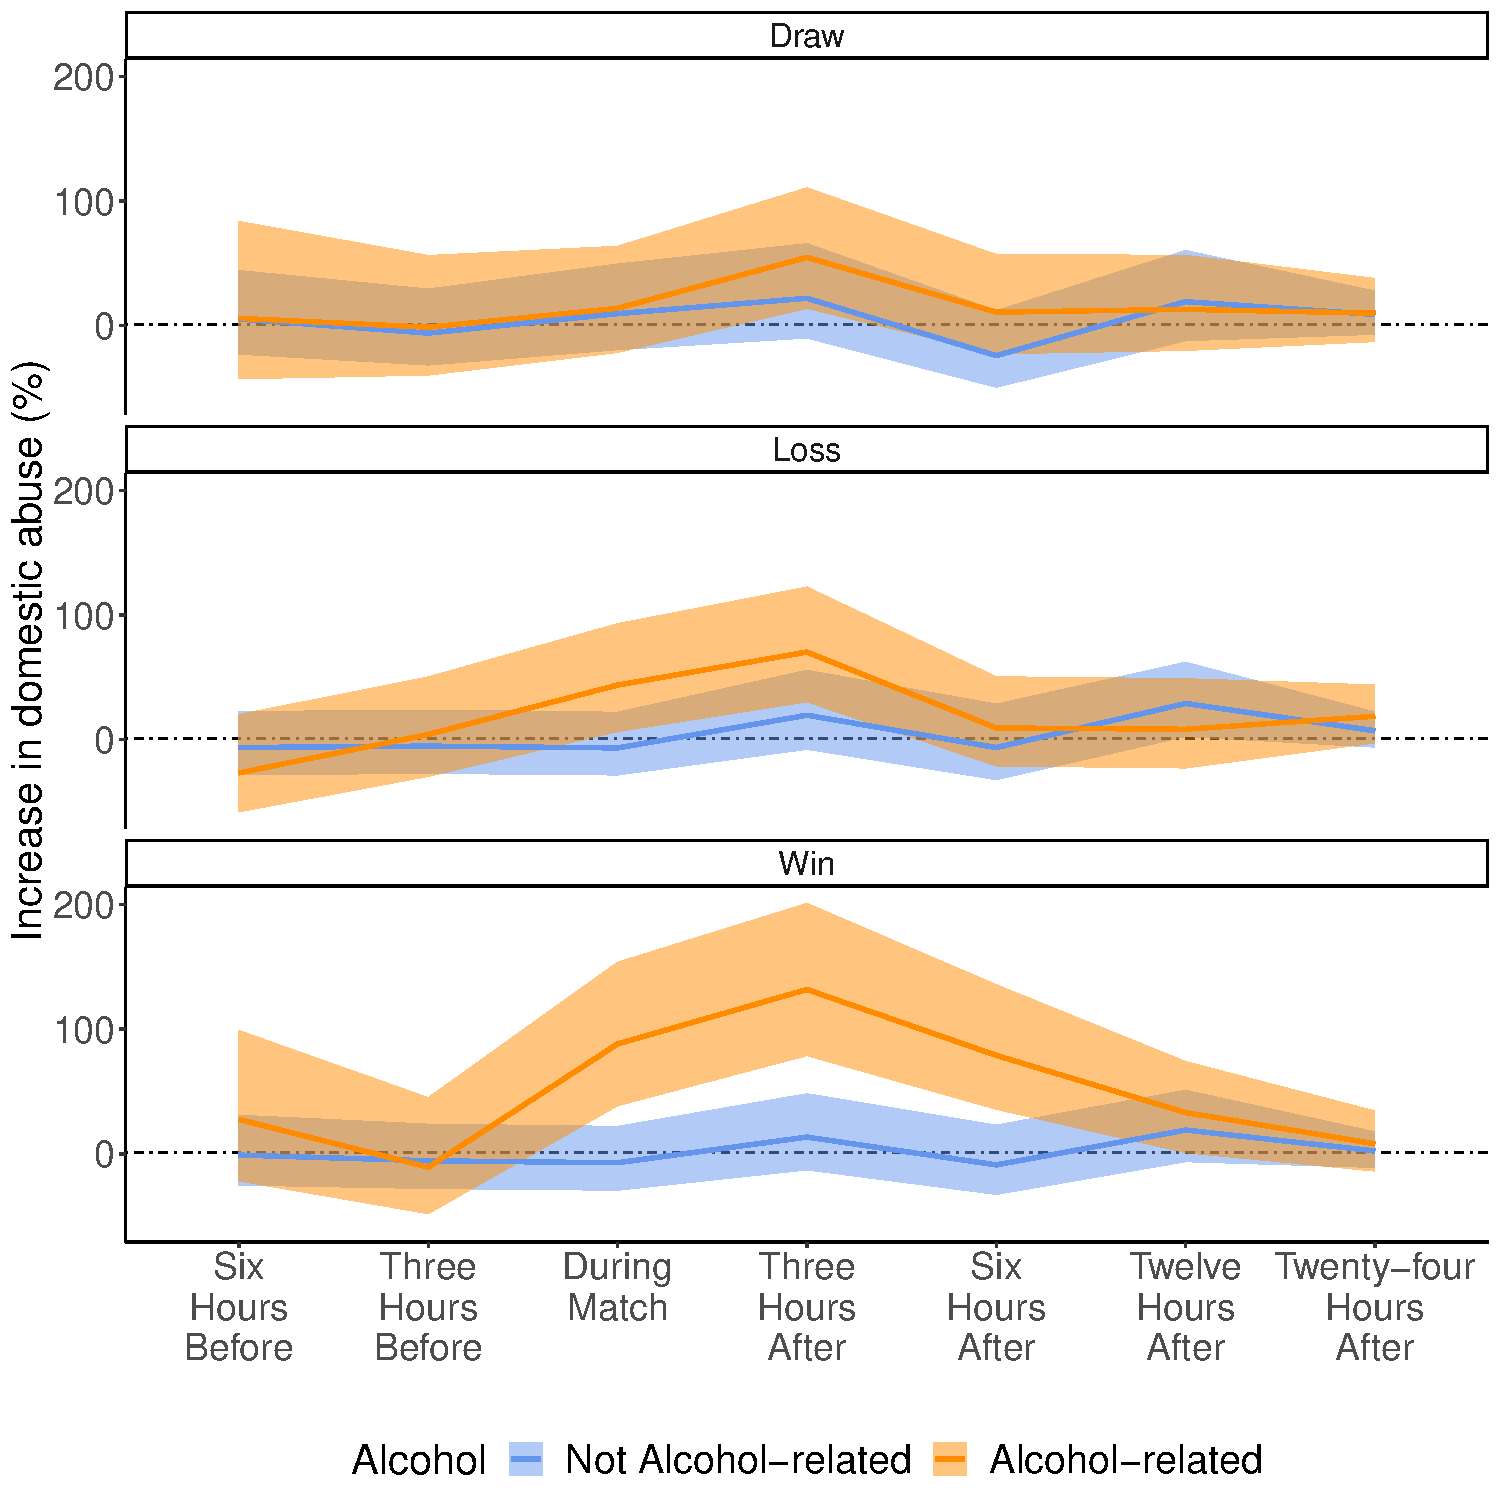
\includegraphics[width=0.75\textwidth]{Threehours_newdata.pdf}
\label{fig:threehours}
		\floatfoot{Note: Estimates are from two separate negative binomial regressions with year, month, day of week, three-hour period of day, Christmas, New Year's eve controls. Shaded area is 95\% CIs.}
\end{figure}
 
To explore whether this increase could be the consequence of an England victory, we exploited the detailed time information in our dataset, which allowed us to conduct a three-hour analysis to explore the more granular temporal patterns of domestic abuse cases (alcohol-related or not) perpetrated before and after an England match.  Figure \ref{fig:threehours} shows a plot of the estimated percentage increase from two negative binomial regressions, revealing a stark increase in alcohol-related domestic abuse on days of an England victory, starting in the three hour period of the match, peaking in the three-hour period afterwards, and gradually declining to its original level in the twenty-four hours following the victory. While a similar pattern can be observed on days when England lost, the increase in the number of alcohol-related cases is substantially smaller and not statistically different from zero. Given that the end time of any given match can vary greatly in the three-hour period (e.g., some of the matches end in the middle of the three-hour interval, therefore any increase in the number of cases in the 1.5 hours following these matches will be captured by the During Match coefficient), it is hard to disentangle the effect by the exact time period, but Figure \ref{fig:threehours} suggests that the increase is the strongest in the hours following the victory. 
 
 Next, we repeated the count per day analyses by offender-victim gender subgroup. Table \ref{gender} in the Appendix shows the results by alcohol-involvement and offender-victim gender group (male to female, female to male, male to male, female to female), on a sample of domestic abuse cases with one victim and offender, where gender information is available (about 86\% of all domestic abuse cases in our dataset). We find a 41\%, 95\% CI [18\%--69\%], increase in the group of alcohol-related male to female cases on England win days, and in the same group we also see some evidence for a smaller, 17\%, 95\% CI [5\%--31\%] increase on days following and England match.



\subsection{Other types of crimes and incidents}


Our rich crime dataset further allows us to explore whether England games have similar effects on other types of criminal behaviours, apart from domestic abuse. Specifically, we examine the effect on England football days on the number of reported property- and hate-related crimes, as well as other violent crimes, after excluding domestic abuse cases. Table \ref{othercrimes} shows the results for these three types of criminal behaviours, by alcohol-involvement. The results reveal a 47\%, 95\% CI [19\%--83\%] increase in the number of non-domestic, alcohol-related violent crimes on England win days.


%  \begin{sidewaystable}[htp]
%\centering
% \caption{The effect of England football days on hate-related, property-related, and other violent offences by alcohol-involvement}
%   \label{othercrimes}
%    \scalebox{0.9}{
% \begin{threeparttable}
%\begin{tabular}{@{\extracolsep{1pt}}lcccccc} 
%\\[-1.8ex]\hline 
%\hline \\[-1.8ex] 
% & \multicolumn{6}{c}{\textit{Dependent variable:}} \\ 
%   & \multicolumn{6}{c}{Number of cases} \\ 
%  & \multicolumn{3}{c}{Non-alcohol related} &\multicolumn{3}{c}{Alcohol-related} \\
%\cline{2-7} 
%\\[-1.8ex] & Hate- & Property- & Other & Hate- & Property & Other \\ & related & related & violent & related & related & violent \\ 
%\\[-1.8ex] & (1) & (2) & (3) & (4) & (5) & (6)\\ 
%\hline \\[-1.8ex] 
%  Tournament on & 1.120$^{**}$ & 1.014 & 1.035 & 1.099 & 1.099$^{*}$ & 1.060 \\ 
%  & [1.030, 1.216] & [0.986, 1.043] & [0.986, 1.085] & [0.914, 1.316] & [1.011, 1.194] & [0.987, 1.139] \\ 
%  & & & & & & \\ 
% England win & 1.002 & 0.961 & 1.085 & 1.556 & 1.291 & 1.473$^{***}$ \\ 
%  & [0.759, 1.311] & [0.879, 1.052] & [0.935, 1.263] & [0.902, 2.558] & [0.998, 1.662] & [1.192, 1.826] \\ 
%  & & & & & & \\ 
% England draw & 0.993 & 0.953 & 0.970 & 0.848 & 0.934 & 1.251 \\ 
%  & [0.709, 1.369] & [0.859, 1.059] & [0.810, 1.167] & [0.400, 1.624] & [0.701, 1.237] & [0.974, 1.613] \\ 
%  & & & & & & \\ 
% England lost & 0.984 & 0.974 & 1.066 & 0.760 & 1.008 & 0.988 \\ 
%  & [0.744, 1.288] & [0.890, 1.066] & [0.917, 1.243] & [0.363, 1.427] & [0.744, 1.353] & [0.785, 1.247] \\ 
%  & & & & & & \\ 
% After England & 1.124 & 0.978 & 1.085 & 1.244 & 1.047 & 1.092 \\ 
%  & [0.953, 1.323] & [0.925, 1.035] & [0.988, 1.193] & [0.872, 1.742] & [0.884, 1.237] & [0.948, 1.258] \\
%
% % & & & & & & \\ 
%\hline \\[-1.8ex] 
%Observations & 3,570 & 3,570 & 3,570 & 3,570 & 3,570 & 3,570 \\ 
%%Log Likelihood & $-$9,086.944 & $-$15,273.310 & $-$14,697.050 & $-$5,347.670 & $-$8,646.912 & $-$11,171.590 \\ 
%%$\theta$ & 23.936$^{***}$  (2.255) & 110.360$^{***}$  (4.838) & 29.145$^{***}$  (0.972) & 9.774$^{***}$  (1.829) & 30.885$^{***}$  (3.014) & 18.765$^{***}$  (0.926) \\ 
%%Akaike Inf. Crit. & 18,241.890 & 30,614.620 & 29,462.100 & 10,763.340 & 17,361.830 & 22,411.180 \\ 
%\hline 
%\hline \\[-1.8ex] 
%\textit{Note:}  & \multicolumn{6}{r}{$^{*}$p$<$0.1; $^{**}$p$<$0.05; $^{***}$p$<$0.01} \\ 
%\end{tabular} 
%\begin{tablenotes}
%      \item[a] \textit{$^{*}$p$<$0.05; $^{**}$p$<$0.01; $^{***}$p$<$0.001}
%      \item[b] \textit{Estimates are exponentiated coefficients from a series of negative binomial regressions with non-match day as benchmark; controls include day of week, month, year, Christmas, and New Year's Eve; 95\% confidence intervals are in square brackets}
%    \end{tablenotes}
%\end{threeparttable} }
%\end{sidewaystable}
%


\begin{sidewaystable}[htp]
\centering
 \caption{The effect of England football days on hate-related, property-related, and other violent offences by alcohol-involvement}
   \label{othercrimes}
    \scalebox{0.9}{
 \begin{threeparttable}
\begin{tabular}{@{\extracolsep{1pt}}lcccccc} 
\\[-1.8ex]\hline 
\hline \\[-1.8ex] 
 & \multicolumn{6}{c}{\textit{Dependent variable:}} \\ 
   & \multicolumn{6}{c}{Number of cases} \\ 
  & \multicolumn{3}{c}{Non-alcohol-related} &\multicolumn{3}{c}{Alcohol-related} \\
\cline{2-7} 
\\[-1.8ex] & Hate- & Property- & Other & Hate- & Property & Other \\ & related & related & violent & related & related & violent \\ 
\\[-1.8ex] & (1) & (2) & (3) & (4) & (5) & (6)\\ 
\hline \\[-1.8ex] 
 Tournament on & 1.120 & 1.014 & 1.035 & 1.099 & 1.099 & 1.060 \\ 
  & [1.030, 1.216] & [0.986, 1.043] & [0.986, 1.085] & [0.914, 1.316] & [1.011, 1.194] & [0.987, 1.139] \\ 
  & (0.008) & (0.323) & (0.165) & (0.309) & (0.027) & (0.110) \\ 
  & & & & & & \\ 
 England win & 1.002 & 0.961 & 1.085 & 1.556 & 1.291 & 1.473$^{*}$ \\ 
  & [0.759, 1.311] & [0.879, 1.052] & [0.935, 1.263] & [0.902, 2.558] & [0.998, 1.662] & [1.192, 1.826] \\ 
  & (0.987) & (0.391) & (0.288) & (0.092) & (0.049) & (0.0004) \\ 
  & & & & & & \\ 
 England draw & 0.993 & 0.953 & 0.970 & 0.848 & 0.934 & 1.251 \\ 
  & [0.709, 1.369] & [0.859, 1.059] & [0.810, 1.167] & [0.400, 1.624] & [0.701, 1.237] & [0.974, 1.613] \\ 
  & (0.967) & (0.373) & (0.747) & (0.642) & (0.636) & (0.082) \\ 
  & & & & & & \\ 
 England lost & 0.984 & 0.974 & 1.066 & 0.760 & 1.008 & 0.988 \\ 
  & [0.744, 1.288] & [0.890, 1.066] & [0.917, 1.243] & [0.363, 1.427] & [0.744, 1.353] & [0.785, 1.247] \\ 
  & (0.908) & (0.562) & (0.411) & (0.426) & (0.956) & (0.922) \\ 
  & & & & & & \\ 
 After England & 1.124 & 0.978 & 1.085 & 1.244 & 1.047 & 1.092 \\ 
  & [0.953, 1.323] & [0.925, 1.035] & [0.988, 1.193] & [0.872, 1.742] & [0.884, 1.237] & [0.948, 1.258] \\ 
  & (0.162) & (0.446) & (0.091) & (0.216) & (0.594) & (0.222) \\ 


 % & & & & & & \\ 
\hline \\[-1.8ex] 
Observations & 3,570 & 3,570 & 3,570 & 3,570 & 3,570 & 3,570 \\ 
%Log Likelihood & $-$9,086.944 & $-$15,273.310 & $-$14,697.050 & $-$5,347.670 & $-$8,646.912 & $-$11,171.590 \\ 
%$\theta$ & 23.936$^{***}$  (2.255) & 110.360$^{***}$  (4.838) & 29.145$^{***}$  (0.972) & 9.774$^{***}$  (1.829) & 30.885$^{***}$  (3.014) & 18.765$^{***}$  (0.926) \\ 
%Akaike Inf. Crit. & 18,241.890 & 30,614.620 & 29,462.100 & 10,763.340 & 17,361.830 & 22,411.180 \\ 
\hline 
\hline \\[-1.8ex] 
%\textit{Note:}  & \multicolumn{6}{r}{$^{*}$p$<$0.1; $^{**}$p$<$0.05; $^{***}$p$<$0.01} \\ 
\end{tabular} 
\begin{tablenotes}
      \item[a] \textit{Estimates are exponentiated coefficients from a series of negative binomial regressions with non-match day as benchmark; controls include day of week, month, year, Christmas, and New Year's Eve; 95\% confidence intervals are in square brackets, p-values are in parentheses}
       \item[b] \textit{Coefficients denoted with $*$ are significant at Bonferroni-corrected alpha levels}
    \end{tablenotes}
\end{threeparttable} }
\end{sidewaystable}



%Compared to non-match days, hate crimes and incidents with no alcohol-involvement increase by 12\%, 95\% CI [3\%--22\%], during the months of the tournaments. 

%Most importantly, the effect of an England win on alcohol-related cases clearly extends to other, non-domestic violent offences, resulting in an almost identical, 47\%, 95\% CI [19\%--83\%], increase compared to non-match days. While it is possible that misclassified domestic abuse cases contribute to this result (e.g, if the victim chooses not to disclose any relationship to the offender), these results suggests that the increase in alcohol-related violence following an England victory is not limited to domestic settings. 

\FloatBarrier


\subsection{Other types of sports: rugby}
%Does this effect generalise to other sporting events, or is it specific to national football tournaments? It has been previously suggested that other popular sports, such as rugby have similar links with domestic abuse \cite{Brooks-Hay2018}. Rugby is the second most popular sport in England after football \cite{Ipsos2003}. Focusing on the Six Nations, a high-profile rugby tournament that takes place every year in the months of February and March with the participation of England, Wales, Scotland, Ireland, France and Italy, we explored whether the reported number of domestic abuse cases increase on days when the England national rugby team plays. 

%Each tournament year, England plays one match with each of the other five participating countries, and these matches take place almost always during the weekend (Saturday, $N = 37$; Sunday, $N = 11$; Friday, $N = 2$). The most common result for England is to win ($N = 35$), much less frequent are losses ($N = 12$), and draws ($N = 2$).


Next, we explore how matches of the England national rugby union team in the Six Nations tournament affect the reported number of alcohol and non-alcohol-related domestic abuse cases. Table \ref{rugby} shows no comparable effects on domestic abuse, alcohol-related or not. 

%potentially stemming from differences in timing, media coverage, audience numbers, and the involvement of alcohol between the two tournaments.


%\begin{table*}[!htbp] \centering 
%  \begin{threeparttable}
%  \caption{The effect of England rugby days (Six Nations) on domestic abuse by alcohol-involvement} 
%  \label{rugby} 
%\begin{tabular}{@{\extracolsep{5pt}}lcc} 
%\\[-1.8ex]\hline 
%\hline \\[-1.8ex] 
% & \multicolumn{2}{c}{\textit{Dependent variable:}} \\ 
%\cline{2-3} 
%\\[-1.8ex] & \multicolumn{2}{c}{Number of cases} \\ 
% & Non-alcohol related & Alcohol-related\\ 
% & domestic abuse & domestic abuse\\
%\\[-1.8ex] & (1) & (2)\\ 
%\hline \\[-1.8ex] 
%Tournament on & 0.980 & 0.969 \\ 
%  & [0.947, 1.014] & [0.923, 1.017] \\ 
%  & & \\ 
% England win & 0.967 & 1.058 \\ 
%  & [0.906, 1.033] & [0.973, 1.151] \\ 
%  & & \\ 
% England draw & 1.030 & 0.966 \\ 
%  & [0.810, 1.318] & [0.716, 1.308] \\ 
%  & & \\ 
% England lost & 1.067 & 0.989 \\ 
%  & [0.963, 1.184] & [0.867, 1.129] \\ 
%  & & \\ 
% After England & 0.983 & 1.004 \\ 
%  & [0.929, 1.041] & [0.931, 1.083] \\ 
%
% % & & \\ 
%\hline \\[-1.8ex] 
%Observations & 3,570 & 3,570 \\ 
%%Log Likelihood & $-$14,692.860 & $-$12,087.270 \\ 
%%$\theta$ & 51.260$^{***}$  (1.967) & 38.539$^{***}$  (2.040) \\ 
%%Akaike Inf. Crit. & 29,453.730 & 24,242.540 \\ 
%\hline 
%\hline \\[-1.8ex] 
%Notes:
%%\textit{Note:}  & \multicolumn{2}{r}{$^{*}$p$<$0.1; $^{**}$p$<$0.05; $^{***}$p$<$0.01} \\ 
%\end{tabular} 
%\begin{tablenotes}
%      \item[a] \textit{$^{*}$p$<$0.05; $^{**}$p$<$0.01; $^{***}$p$<$0.001}
%      \item[b] \textit{Estimates are exponentiated coefficients from negative binomial regressions with non-match day as benchmark; controls include day of week, month, year, Christmas, and New Year's Eve; 95\% confidence intervals are in square brackets}
%    \end{tablenotes}
%\end{threeparttable} 
%\end{table*}



\begin{table*}[!htbp] \centering 
  \begin{threeparttable}
  \caption{The effect of England rugby days (Six Nations) on domestic abuse by alcohol-involvement} 
  \label{rugby} 
\begin{tabular}{@{\extracolsep{5pt}}lcc} 
\\[-1.8ex]\hline 
\hline \\[-1.8ex] 
 & \multicolumn{2}{c}{\textit{Dependent variable:}} \\ 
\cline{2-3} 
\\[-1.8ex] & \multicolumn{2}{c}{Number of cases} \\ 
 & Non-alcohol-related & Alcohol-related\\ 
 & domestic abuse & domestic abuse\\
\\[-1.8ex] & (1) & (2)\\ 
\hline \\[-1.8ex] 
Tournament on & 0.980 & 0.969 \\ 
  & [0.947, 1.014] & [0.923, 1.017] \\ 
  & (0.249) & (0.202) \\ 
  & & \\ 
 England win & 0.967 & 1.058 \\ 
  & [0.906, 1.033] & [0.973, 1.151] \\ 
  & (0.319) & (0.185) \\ 
  & & \\ 
 England draw & 1.030 & 0.966 \\ 
  & [0.810, 1.318] & [0.716, 1.308] \\ 
  & (0.811) & (0.822) \\ 
  & & \\ 
 England lost & 1.067 & 0.989 \\ 
  & [0.963, 1.184] & [0.867, 1.129] \\ 
  & (0.215) & (0.871) \\ 
  & & \\ 
 After England & 0.983 & 1.004 \\ 
  & [0.929, 1.041] & [0.931, 1.083] \\ 
  & (0.565) & (0.917) \\ 
 % & & \\ 
\hline \\[-1.8ex] 
Observations & 3,570 & 3,570 \\ 
%Log Likelihood & $-$14,692.860 & $-$12,087.270 \\ 
%$\theta$ & 51.260$^{***}$  (1.967) & 38.539$^{***}$  (2.040) \\ 
%Akaike Inf. Crit. & 29,453.730 & 24,242.540 \\ 
\hline 
\hline \\[-1.8ex] 
Notes:
%\textit{Note:}  & \multicolumn{2}{r}{$^{*}$p$<$0.1; $^{**}$p$<$0.05; $^{***}$p$<$0.01} \\ 
\end{tabular} 
\begin{tablenotes}
      \item[a] \textit{Estimates are exponentiated coefficients from negative binomial regressions with non-match day as benchmark; controls include day of week, month, year, Christmas, and New Year's Eve; 95\% confidence intervals are in square brackets, p-values are in parentheses}
             \item[b] \textit{Coefficients denoted with $*$ are significant at Bonferroni-corrected alpha levels}

    \end{tablenotes}
\end{threeparttable} 
\end{table*}


\FloatBarrier


\subsection{Previous evidence and robustness checks}


A previous study by \citeA{Kirby2014} found that an England loss results in the most pronounced increase in domestic abuse (38\%), while a win or draw have a slightly smaller effect (26\%). They used daily counts of IPV in Lancashire from the months of the 2002, 2006, 2010 World Cups. Upon re-analysing their data by treating wins and draws as two separate variables (see Table \ref{kirbyrep1}), we estimate a 45\%, 95\% CI [28\%--64\%], increase on England win days, and a 39\%, 95\% CI [18\%--64\%], increase on England loss days, and no effect when England draws. Separating wins and draws clearly improves the fit of the model, demonstrated by the reduction in the Bayesian and Akaike Information Criteria (BIC and AIC, respectively). The estimated effect of an England loss is insensitive to this change. 


%\begin{table*}[!htbp]
%\centering
% \caption{Re-analysis of Kirby et al. (2014) with wins and draws as separate variables}
%   \label{kirbyrep1}
%   \scalebox{0.85}{
% \begin{threeparttable}
%\begin{tabular}{@{\extracolsep{5pt}}lcc} 
%\\[-1.8ex]\hline 
%\hline \\[-1.8ex] 
% & \multicolumn{2}{c}{\textit{Dependent variable:}} \\ 
%\cline{2-3} 
%\\[-1.8ex] & \multicolumn{2}{c}{Number of reported Intimate Partner Violence cases per day} \\ 
%\\ 
%  & Original Model & Win/Draw Separate \\ 
%\\[-1.8ex] & (1) & (2)\\ 
%\hline \\[-1.8ex] 
% England windraw & 1.256$^{***}$ &  \\ 
%  & [1.128, 1.398] &  \\ 
%  England win &  & 1.452$^{***}$ \\ 
%  &  & [1.282, 1.644] \\ 
%  England draw &  & 1.032 \\ 
%  &  & [0.893, 1.191] \\ 
%  England lost & 1.382$^{***}$ & 1.388$^{***}$ \\ 
%  & [1.151, 1.662] & [1.175, 1.639] \\ 
%  After England & 1.111$^{*}$ & 1.113$^{*}$ \\ 
%  & [1.004, 1.228] & [1.014, 1.221] \\ 
%%  Constant & 41.905 & 41.561 \\ 
%%  & (37.378, 46.946) & (37.349, 46.200) \\ 
% \hline \\[-1.8ex] 
%Observations & 92 & 92 \\ 
%BIC & 747.763 & 739.662 \\ 
%AIC & 714.980 & 704.356 \\ 
%\hline 
%\hline \\[-1.8ex] 
%\end{tabular} 
%\begin{tablenotes}
%      \item[a] \textit{$^{*}$p$<$0.05; $^{**}$p$<$0.01; $^{***}$p$<$0.001}
%      \item[b] \textit{Estimates are exponentiated coefficients from negative binomial regressions (based on tests of overdispersion) with year and day of week controls and no England match days during the tournament as benchmark; data is only available during the tournament period; 95\% confidence intervals are in square brackets}
%    \end{tablenotes}
%\end{threeparttable} }
%\end{table*}


\begin{table*}[!htbp]
\centering
 \caption{Re-analysis of Kirby et al. (2014) with wins and draws as separate variables}
   \label{kirbyrep1}
   \scalebox{0.85}{
 \begin{threeparttable}
\begin{tabular}{@{\extracolsep{5pt}}lcc} 
\\[-1.8ex]\hline 
\hline \\[-1.8ex] 
 & \multicolumn{2}{c}{\textit{Dependent variable:}} \\ 
\cline{2-3} 
\\[-1.8ex] & \multicolumn{2}{c}{Number of reported Intimate Partner Violence cases per day} \\ 
\\ 
  & Original Model & Win/Draw Separate \\ 
\\[-1.8ex] & (1) & (2)\\ 
\hline \\[-1.8ex] 
England windraw & 1.256$^{*}$ &  \\ 
  & [1.128, 1.398] &  \\ 
  & (0.00004) &  \\ 
  England win &  & 1.452$^{*}$ \\ 
  &  & [1.282, 1.644] \\ 
  &  & (0.000) \\ 
    England draw &  & 1.032 \\ 
  &  & [0.893, 1.191] \\ 
  &  & (0.671) \\
  England lost & 1.382$^{*}$ & 1.388$^{*}$ \\ 
  & [1.151, 1.662] & [1.175, 1.639] \\ 
  & (0.001) & (0.0002) \\ 
  After England & 1.111 & 1.113 \\ 
  & [1.004, 1.228] & [1.014, 1.221] \\ 
  & (0.042) & (0.024) \\  
%  England lost &  & 1.388 \\ 
%  &  & [1.175, 1.639] \\ 
%  &  & (0.0002) \\ 
%  After England &  & 1.113 \\ 
%  &  & [1.014, 1.221] \\ 
%  &  & (0.024) \\ 

 \hline \\[-1.8ex] 
Observations & 92 & 92 \\ 
BIC & 747.763 & 739.662 \\ 
AIC & 714.980 & 704.356 \\ 
\hline 
\hline \\[-1.8ex] 
\end{tabular} 
\begin{tablenotes}
%      \item[a] \textit{$^{*}$p$<$0.05; $^{**}$p$<$0.01; $^{***}$p$<$0.001}
      \item[a] \textit{Estimates are exponentiated coefficients from negative binomial regressions (based on tests of overdispersion) with year and day of week controls and no England match days during the tournament as benchmark; data is only available during the tournament period; 95\% confidence intervals are in square brackets, p-values are in parentheses}
                   \item[b] \textit{Coefficients denoted with $*$ are significant at Bonferroni-corrected alpha levels}
    \end{tablenotes}
\end{threeparttable} }
\end{table*}


To further probe the robustness of the results, we find it instructive to break our analysis into specific tournament years using both datasets (Lancashire and West Midlands; see Table \ref{kirbyrep2}). To be consistent with previous results, we present the regressions for both types of domestic abuse (alcohol and non-alcohol-related), however, unfortunately we cannot do the same for the Lancashire dataset, as it contains no information on alcohol-involvement. Only year 2010 overlaps in the two datasets, which allows us to (at least partly) evaluate the robustness of our results. 



%To explore the underlying reason for this discrepancy and test the robustness of our results, we find it instructive to break our analysis into specific tournament years using both datasets (Lancashire and West Midlands; see Table \ref{kirbyrep2}). To be consistent with previous results, we present the regressions for both types of domestic abuse (alcohol and non-alcohol-related), however, unfortunately we cannot do the same for the Lancashire dataset, as it contains no information on alcohol-involvement. Only year 2010 overlaps in the two datasets, which allows us to (at least partly) evaluate the robustness of our results.

An apparent common pattern in both datasets is the large effect of England's victory over Slovenia in the group stage of the 2010 World Cup, which, after much anticipation, secured their progression to the next stage of the tournament: on the same day, we estimate a 91\%, 95\% CI [53\%--139\%] increase in the number of domestic abuse cases reported in Lancashire, and a 84\%, 95\% CI [31\%--160\%], increase in the number of alcohol-related domestic abuse cases reported in the West Midlands. 

Equally, the subsequent loss against Germany in the knockout stage in the same resulted in a substantial increase in the number of reported domestic abuse incidents: on the same day, we estimate a 57\%, 95\% CI [27\%--93\%] increase in the number of domestic abuse cases reported in Lancashire, and a smaller, 43\%, 95\% CI [4\%--100\%], increase in the number of alcohol-related domestic abuse cases reported in the West Midlands.



%In addition, the size of the win and loss coefficients are remarkably similar, giving us confidence that these effects are likely to generalise to other areas within England. These patterns are also in line with findings from an earlier examination by \cite{Brimicombe2012}, who found an increase in the number of domestic abuse cases reported to the police across England on both victory and loss days during the 2010 World Cup.  Most importantly, if the same mechanism lies behind our results, then it suggests that the increase observed in other datasets is also likely to stem from alcohol-related cases. 
   
  It is also clear that World Cup wins have the strongest effect on the number of domestic abuse incidents: a clear, large increase can be observed in 2002, 2006, 2010, and 2018 (England did not have a single victory in the 2014 World Cup).
 

%\newpage



%\begin{sidewaystable}[!htbp]
%\centering
% \caption{The effect of England football days on domestic abuse by alcohol-involvement and tournament, Lancashire and West Midlands data}
%   \label{kirbyrep2}
%    \scalebox{0.65}{
% \begin{threeparttable}
%\begin{tabular}{@{\extracolsep{1pt}}lccccccccccccc} 
%\\[-1.8ex]\hline 
%\hline \\[-1.8ex] 
% & \multicolumn{13}{c}{\textit{Dependent variable:}} \\ 
%\cline{2-14} 
%& \multicolumn{13}{c}{Number of domestic abuse cases} \\ 
%\\[-1.8ex] & \multicolumn{3}{c}{Lancashire} & \multicolumn{10}{c}{West Midlands} \\ 
%\\[-1.8ex] & \multicolumn{1}{c}{All\textsuperscript{c}} & \multicolumn{1}{c}{All} & \multicolumn{1}{c}{All} & \multicolumn{1}{c}{NA\textsuperscript{c}} & \multicolumn{1}{c}{A\textsuperscript{c}} & \multicolumn{1}{c}{NA} & \multicolumn{1}{c}{A} & \multicolumn{1}{c}{NA} & \multicolumn{1}{c}{A} & \multicolumn{1}{c}{NA} & \multicolumn{1}{c}{A} & \multicolumn{1}{c}{NA} & \multicolumn{1}{c}{A} \\ 
%% & \textit{binomial} & \multicolumn{2}{c}{\textit{}} & \multicolumn{10}{c}{\textit{binomial}} \\ 
% \\[-1.8ex] & 2002 & 2006 & 2010 & 2010 & 2010 & 2012 & 2012 & 2014 & 2014 & 2016 & 2016 & 2018 & 2018  \\ 
%\\[-1.8ex] & (1) & (2) & (3) & (4) & (5) & (6) & (7) & (8) & (9) & (10) & (11) & (12) & (13)\\ 
%\hline \\[-1.8ex] 
%Tournament on &  &  &  & 1.047 & 1.038 & 0.881 & 0.936 & 0.976 & 0.999 & 1.041 & 0.855$^{*}$ & 1.081 & 1.014 \\ 
%  &  &  &  & [0.974, 1.127] & [0.936, 1.151] & [0.740, 1.049] & [0.780, 1.125] & [0.901, 1.057] & [0.890, 1.123] & [0.962, 1.128] & [0.757, 0.967] & [0.979, 1.194] & [0.889, 1.155] \\ 
%  England win & 1.596$^{**}$ & 1.297$^{***}$ & 1.916$^{***}$ & 1.171 & 1.845$^{***}$ & 0.673$^{*}$ & 1.106 &  &  & 1.062 & 1.302 & 1.006 & 1.529$^{***}$ \\ 
%  & [1.186, 2.153] & [1.115, 1.505] & [1.528, 2.389] & [0.897, 1.514] & [1.310, 2.595] & [0.456, 0.982] & [0.770, 1.576] &  &  & [0.796, 1.420] & [0.834, 1.995] & [0.844, 1.202] & [1.249, 1.869] \\ 
%  England draw & 1.100 & 1.098 & 0.863 & 0.905 & 1.248 & 1.204 & 1.116 & 0.984 & 0.954 & 1.069 & 1.128 &  &  \\ 
%  & [0.820, 1.477] & [0.802, 1.481] & [0.713, 1.037] & [0.736, 1.107] & [0.966, 1.611] & [0.773, 1.877] & [0.676, 1.805] & [0.723, 1.343] & [0.576, 1.527] & [0.869, 1.318] & [0.835, 1.517] &  &  \\ 
%  England lost & 1.200 & 1.373$^{**}$ & 1.568$^{***}$ & 1.082 & 1.435$^{*}$ & 0.812 & 0.961 & 0.934 & 1.079 & 0.772 & 0.620 & 1.101 & 1.252 \\ 
%  & [0.759, 1.894] & [1.086, 1.721] & [1.270, 1.928] & [0.838, 1.389] & [1.036, 1.992] & [0.508, 1.293] & [0.614, 1.491] & [0.747, 1.170] & [0.792, 1.459] & [0.568, 1.048] & [0.343, 1.058] & [0.904, 1.348] & [0.975, 1.603] \\ 
%  After England & 1.253$^{*}$ & 1.122 & 1.024 & 1.049 & 1.132 & 0.814 & 1.108 & 1.037 & 1.080 & 1.013 & 0.960 & 1.147$^{*}$ & 1.390$^{***}$ \\ 
%  & [1.029, 1.526] & [0.977, 1.286] & [0.900, 1.162] & [0.907, 1.212] & [0.928, 1.380] & [0.617, 1.070] & [0.842, 1.453] & [0.863, 1.249] & [0.832, 1.394] & [0.864, 1.188] & [0.750, 1.224] & [1.001, 1.317] & [1.173, 1.646] \\
%
% \hline \\[-1.8ex] 
%Observations & 30 & 32 & 30 & 365 & 365 & 366 & 366 & 365 & 365 & 366 & 366 & 365 & 365 \\ 
%%Log Likelihood & $-$112.494 & $-$101.847 & $-$107.268 & $-$1,344.208 & $-$1,305.710 & $-$1,294.898 & $-$1,189.726 & $-$1,494.583 & $-$1,175.810 & $-$1,503.841 & $-$1,197.151 & $-$1,594.487 & $-$1,200.743 \\ 
%%$\theta$ & 57.581$^{*}$  (31.978) &  &  & 215.538$^{***}$  (65.249) & 76.028$^{***}$  (16.053) & 43.908$^{***}$  (6.783) & 55.674$^{***}$  (12.862) & 75.808$^{***}$  (9.733) & 72.582$^{***}$  (18.248) & 90.546$^{***}$  (12.118) & 69.058$^{***}$  (16.506) & 49.787$^{***}$  (5.114) & 64.954$^{***}$  (15.073) \\ 
%%Akaike Inf. Crit. & 246.989 & 225.694 & 236.536 & 2,738.415 & 2,661.420 & 2,639.797 & 2,429.452 & 3,037.165 & 2,399.621 & 3,057.682 & 2,444.301 & 3,236.974 & 2,449.485 \\ 
%\hline 
%\hline \\[-1.8ex] 
%%\textit{Note:}  & \multicolumn{13}{r}{$^{*}$p$<$0.1; $^{**}$p$<$0.05; $^{***}$p$<$0.01} \\ 
%\end{tabular} 
%\begin{tablenotes}
%      \item[a] \textit{$^{*}$p$<$0.05; $^{**}$p$<$0.01; $^{***}$p$<$0.001}
%      \item[b] \textit{Estimates are exponentiated coefficients from a series of negative binomial regressions, except for Model (2) and (3) which are from Poisson regressions (based on tests of overdispersion). Each regression is restricted to a specific tournament year. Regressions 1-3 have day of week control with non England tournament days as benchmark, regressions 4-13 have month, day of week, Christmas, New Year's eve controls, with non-match days as benchmark; 95\% confidence intervals are in square brackets}
%      \item[c] \textit{All = All cases, NA = Non-alcohol related cases, A = Alcohol-related cases}
%    \end{tablenotes}
%\end{threeparttable} }
%\end{sidewaystable}



\begin{sidewaystable}[!htbp]
\centering
 \caption{The effect of England football days on domestic abuse by alcohol-involvement and tournament, Lancashire and West Midlands data}
   \label{kirbyrep2}
    \scalebox{0.65}{
 \begin{threeparttable}
\begin{tabular}{@{\extracolsep{1pt}}lccccccccccccc} 
\\[-1.8ex]\hline 
\hline \\[-1.8ex] 
 & \multicolumn{13}{c}{\textit{Dependent variable:}} \\ 
\cline{2-14} 
& \multicolumn{13}{c}{Number of domestic abuse cases} \\ 
\\[-1.8ex] & \multicolumn{3}{c}{Lancashire} & \multicolumn{10}{c}{West Midlands} \\ 
\\[-1.8ex] & \multicolumn{1}{c}{All\textsuperscript{c}} & \multicolumn{1}{c}{All} & \multicolumn{1}{c}{All} & \multicolumn{1}{c}{NA\textsuperscript{c}} & \multicolumn{1}{c}{A\textsuperscript{c}} & \multicolumn{1}{c}{NA} & \multicolumn{1}{c}{A} & \multicolumn{1}{c}{NA} & \multicolumn{1}{c}{A} & \multicolumn{1}{c}{NA} & \multicolumn{1}{c}{A} & \multicolumn{1}{c}{NA} & \multicolumn{1}{c}{A} \\ 
% & \textit{binomial} & \multicolumn{2}{c}{\textit{}} & \multicolumn{10}{c}{\textit{binomial}} \\ 
 \\[-1.8ex] & 2002 & 2006 & 2010 & 2010 & 2010 & 2012 & 2012 & 2014 & 2014 & 2016 & 2016 & 2018 & 2018  \\ 
\\[-1.8ex] & (1) & (2) & (3) & (4) & (5) & (6) & (7) & (8) & (9) & (10) & (11) & (12) & (13)\\ 
\hline \\[-1.8ex] 
Tournament on &  &  &  & 1.047 & 1.038 & 0.881 & 0.936 & 0.976 & 0.999 & 1.041 & 0.855 & 1.081 & 1.014 \\ 
  &  &  &  & [0.974, 1.127] & [0.936, 1.151] & [0.740, 1.049] & [0.780, 1.125] & [0.901, 1.057] & [0.890, 1.123] & [0.962, 1.128] & [0.757, 0.967] & [0.979, 1.194] & [0.889, 1.155] \\ 
  &  &  &  & (0.216) & (0.481) & (0.176) & (0.491) & (0.547) & (0.992) & (0.321) & (0.013) & (0.126) & (0.839) \\ 
  England win & 1.596$^{*}$ & 1.297$^{*}$ & 1.916$^{*}$ & 1.171 & 1.845$^{*}$ & 0.673 & 1.106 &  &  & 1.062 & 1.302 & 1.006 & 1.529$^{*}$ \\ 
  & [1.186, 2.153] & [1.115, 1.505] & [1.528, 2.389] & [0.897, 1.514] & [1.310, 2.595] & [0.456, 0.982] & [0.770, 1.576] &  &  & [0.796, 1.420] & [0.834, 1.995] & [0.844, 1.202] & [1.249, 1.869] \\ 
  & (0.003) & (0.001) & (0.000) & (0.238) & (0.0005) & (0.045) & (0.582) &  &  & (0.685) & (0.235) & (0.951) & (0.00004) \\ 
  England draw & 1.100 & 1.098 & 0.863 & 0.905 & 1.248 & 1.204 & 1.116 & 0.984 & 0.954 & 1.069 & 1.128 &  &  \\ 
  & [0.820, 1.477] & [0.802, 1.481] & [0.713, 1.037] & [0.736, 1.107] & [0.966, 1.611] & [0.773, 1.877] & [0.676, 1.805] & [0.723, 1.343] & [0.576, 1.527] & [0.869, 1.318] & [0.835, 1.517] &  &  \\ 
  & (0.525) & (0.550) & (0.121) & (0.337) & (0.090) & (0.414) & (0.661) & (0.918) & (0.851) & (0.528) & (0.432) &  &  \\ 
  England lost & 1.200 & 1.373 & 1.568$^{*}$ & 1.082 & 1.435 & 0.812 & 0.961 & 0.934 & 1.079 & 0.772 & 0.620 & 1.101 & 1.252 \\ 
  & [0.759, 1.894] & [1.086, 1.721] & [1.270, 1.928] & [0.838, 1.389] & [1.036, 1.992] & [0.508, 1.293] & [0.614, 1.491] & [0.747, 1.170] & [0.792, 1.459] & [0.568, 1.048] & [0.343, 1.058] & [0.904, 1.348] & [0.975, 1.603] \\ 
  & (0.434) & (0.007) & (0.00003) & (0.540) & (0.031) & (0.384) & (0.861) & (0.550) & (0.626) & (0.097) & (0.095) & (0.343) & (0.075) \\ 
  After England & 1.253 & 1.122 & 1.024 & 1.049 & 1.132 & 0.814 & 1.108 & 1.037 & 1.080 & 1.013 & 0.960 & 1.147 & 1.390$^{*}$ \\ 
  & [1.029, 1.526] & [0.977, 1.286] & [0.900, 1.162] & [0.905, 1.194] & [0.933, 1.331] & [0.535, 1.092] & [0.834, 1.381] & [0.863, 1.249] & [0.832, 1.394] & [0.853, 1.172] & [0.715, 1.206] & [1.001, 1.317] & [1.173, 1.646] \\ 
  & (0.026) & (0.100) & (0.718) & (0.515) & (0.223) & (0.147) & (0.464) & (0.697) & (0.561) & (0.878) & (0.746) & (0.051) & (0.0002) \\


 \hline \\[-1.8ex] 
Observations & 30 & 32 & 30 & 365 & 365 & 366 & 366 & 365 & 365 & 366 & 366 & 365 & 365 \\ 
%Log Likelihood & $-$112.494 & $-$101.847 & $-$107.268 & $-$1,344.208 & $-$1,305.710 & $-$1,294.898 & $-$1,189.726 & $-$1,494.583 & $-$1,175.810 & $-$1,503.841 & $-$1,197.151 & $-$1,594.487 & $-$1,200.743 \\ 
%$\theta$ & 57.581$^{*}$  (31.978) &  &  & 215.538$^{***}$  (65.249) & 76.028$^{***}$  (16.053) & 43.908$^{***}$  (6.783) & 55.674$^{***}$  (12.862) & 75.808$^{***}$  (9.733) & 72.582$^{***}$  (18.248) & 90.546$^{***}$  (12.118) & 69.058$^{***}$  (16.506) & 49.787$^{***}$  (5.114) & 64.954$^{***}$  (15.073) \\ 
%Akaike Inf. Crit. & 246.989 & 225.694 & 236.536 & 2,738.415 & 2,661.420 & 2,639.797 & 2,429.452 & 3,037.165 & 2,399.621 & 3,057.682 & 2,444.301 & 3,236.974 & 2,449.485 \\ 
\hline 
\hline \\[-1.8ex] 
%\textit{Note:}  & \multicolumn{13}{r}{$^{*}$p$<$0.1; $^{**}$p$<$0.05; $^{***}$p$<$0.01} \\ 
\end{tabular} 
\begin{tablenotes}
%      \item[a] \textit{$^{*}$p$<$0.05; $^{**}$p$<$0.01; $^{***}$p$<$0.001}
      \item[a] \textit{Estimates are exponentiated coefficients from a series of negative binomial regressions, except for Model (2) and (3) which are from Poisson regressions (based on tests of overdispersion). Each regression is restricted to a specific tournament year. Regressions 1-3 have day of week control with non England tournament days as benchmark, regressions 4-13 have month, day of week, Christmas, New Year's eve controls, with non-match days as benchmark; 95\% confidence intervals are in square brackets, p-values are in parentheses}
      \item[b] \textit{Coefficients denoted with $*$ are significant at Bonferroni-corrected alpha levels}
      \item[c] \textit{All = All cases, NA = Non-alcohol-related cases, A = Alcohol-related cases}
    \end{tablenotes}
\end{threeparttable} }
\end{sidewaystable}

%
%
%
%\begin{sidewaystable}[!htbp]
%\centering
% \caption{Robustness of the result: sensitivity to the exclusion of specific years}
%  \label{robustness}
% \scalebox{0.8}{
%  \begin{threeparttable}
%\begin{tabular}{@{\extracolsep{5pt}}lcccccccccc} 
%\\[-1.8ex]\hline 
%\hline \\[-1.8ex] 
% & \multicolumn{10}{c}{\textit{Dependent variable:}} \\ 
%\cline{2-11} 
%\\[-1.8ex] & \multicolumn{10}{c}{Number of domestic abuse cases} \\ 
%\\[-1.8ex] & \multicolumn{1}{c}{NA\textsuperscript{c}} & \multicolumn{1}{c}{A\textsuperscript{c}} &  \multicolumn{1}{c}{NA} & \multicolumn{1}{c}{A} &  \multicolumn{1}{c}{NA} & \multicolumn{1}{c}{A} &  \multicolumn{1}{c}{NA} & \multicolumn{1}{c}{A} &  \multicolumn{1}{c}{NA} & \multicolumn{1}{c}{A}  \\
% \\[-1.8ex] & 2010 & 2010 & 2012 & 2012 & 2014 & 2014 & 2016 & 2016 & 2018 & 2018  \\ 
%\\[-1.8ex] & (1) & (2) & (3) & (4) & (5) & (6) & (7) & (8) & (9) & (10)\\ 
%\hline \\[-1.8ex] 
%Tournament on & 1.010 & 0.970 & 1.040$^{*}$ & 0.990 & 1.025 & 0.972 & 1.023 & 1.010 & 1.014 & 0.980 \\ 
%  & [0.968, 1.055] & [0.915, 1.029] & [1.001, 1.081] & [0.937, 1.046] & [0.980, 1.071] & [0.917, 1.031] & [0.980, 1.069] & [0.954, 1.070] & [0.973, 1.057] & [0.926, 1.036] \\ 
%  England win & 0.913 & 1.387$^{***}$ & 1.015 & 1.557$^{***}$ & 0.955 & 1.470$^{***}$ & 0.927 & 1.490$^{***}$ & 0.931 & 1.438$^{**}$ \\ 
%  & [0.798, 1.047] & [1.175, 1.639] & [0.892, 1.157] & [1.312, 1.850] & [0.842, 1.084] & [1.260, 1.716] & [0.809, 1.064] & [1.265, 1.757] & [0.770, 1.126] & [1.149, 1.800] \\ 
%  England draw & 1.091 & 1.143 & 1.027 & 1.141 & 1.050 & 1.173 & 1.022 & 1.134 & 1.034 & 1.134 \\ 
%  & [0.915, 1.304] & [0.904, 1.443] & [0.888, 1.191] & [0.940, 1.386] & [0.895, 1.235] & [0.966, 1.426] & [0.851, 1.231] & [0.907, 1.418] & [0.896, 1.195] & [0.944, 1.362] \\ 
%  England lost & 1.012 & 1.093 & 1.047 & 1.153 & 1.036 & 1.129 & 1.067 & 1.200$^{*}$ & 0.977 & 1.049 \\ 
%  & [0.888, 1.155] & [0.918, 1.301] & [0.929, 1.182] & [0.974, 1.366] & [0.900, 1.194] & [0.941, 1.355] & [0.937, 1.217] & [1.015, 1.420] & [0.835, 1.145] & [0.859, 1.283] \\ 
%  After England & 1.046 & 1.203$^{**}$ & 1.094$^{*}$ & 1.185$^{**}$ & 1.051 & 1.189$^{**}$ & 1.059 & 1.225$^{***}$ & 1.012 & 1.093 \\ 
%  & [0.961, 1.138] & [1.077, 1.343] & [1.013, 1.182] & [1.064, 1.319] & [0.968, 1.142] & [1.069, 1.322] & [0.974, 1.154] & [1.098, 1.366] & [0.921, 1.113] & [0.968, 1.235] \\ 
% \hline \\[-1.8ex] 
%Observations & 3,205 & 3,205 & 3,204 & 3,204 & 3,205 & 3,205 & 3,204 & 3,204 & 3,205 & 3,205 \\ 
%%Log Likelihood & $-$15,738.220 & $-$11,006.630 & $-$15,087.610 & $-$11,568.310 & $-$15,673.620 & $-$11,605.220 & $-$15,608.290 & $-$11,602.150 & $-$15,499.280 & $-$11,605.610 \\ 
%%$\theta$ & 7.385$^{***}$  (0.199) & 28.051$^{***}$  (1.404) & %13.075$^{***}$  (0.373) & 17.870$^{***}$  (0.723) & 7.139$^{***}$  (0.191) & 16.977$^{***}$  (0.674) & 7.284$^{***}$  (0.196) & 16.694$^{***}$  (0.660) & 7.692$^{***}$  (0.208) & 16.664$^{***}$  (0.658) \\ 
%%Akaike Inf. Crit. & 31,526.440 & 22,063.270 & 30,225.220 & 23,186.630 & 31,397.250 & 23,260.450 & 31,266.580 & 23,254.290 & 31,048.560 & 23,261.230 \\ 
%\hline 
%\hline \\[-1.8ex] 
%%\textit{Note:}  & \multicolumn{10}{r}{$^{*}$p$<$0.1; $^{**}$p$<$0.05; $^{***}$p$<$0.01} \\ 
%\end{tabular} 
%%\end{table} 
%\begin{tablenotes}
%      \item[a] \textit{$^{*}$p$<$0.05; $^{**}$p$<$0.01; $^{***}$p$<$0.001}
%      \item[b] \textit{Estimates are exponentiated coefficients from a series of negative binomial regressions (based on tests of overdispersion)  with year, month, day of week, Christmas, New Year's eve controls; 95\% confidence intervals are in square brackets}
%      \item[c] \textit{NA = Non-alcohol related cases, A = Alcohol-related cases}
%    \end{tablenotes}
%\end{threeparttable}   }
%\end{sidewaystable}




\begin{sidewaystable}[!htbp]
\centering
 \caption{Robustness of the result: sensitivity to the exclusion of specific years}
  \label{robustness}
 \scalebox{0.8}{
  \begin{threeparttable}
\begin{tabular}{@{\extracolsep{5pt}}lcccccccccc} 
\\[-1.8ex]\hline 
\hline \\[-1.8ex] 
 & \multicolumn{10}{c}{\textit{Dependent variable:}} \\ 
\cline{2-11} 
\\[-1.8ex] & \multicolumn{10}{c}{Number of domestic abuse cases} \\ 
\\[-1.8ex] & \multicolumn{1}{c}{NA\textsuperscript{c}} & \multicolumn{1}{c}{A\textsuperscript{c}} &  \multicolumn{1}{c}{NA} & \multicolumn{1}{c}{A} &  \multicolumn{1}{c}{NA} & \multicolumn{1}{c}{A} &  \multicolumn{1}{c}{NA} & \multicolumn{1}{c}{A} &  \multicolumn{1}{c}{NA} & \multicolumn{1}{c}{A}  \\
 \\[-1.8ex] & 2010 & 2010 & 2012 & 2012 & 2014 & 2014 & 2016 & 2016 & 2018 & 2018  \\ 
\\[-1.8ex] & (1) & (2) & (3) & (4) & (5) & (6) & (7) & (8) & (9) & (10)\\ 
\hline \\[-1.8ex] 
Tournament on & 1.035 & 0.959 & 1.063 & 1.084 & 0.976 & 1.085 & 0.960 & 1.105 & 0.948 & 1.069 \\ 
  & [0.946, 1.133] & [0.901, 1.021] & [0.994, 1.136] & [1.014, 1.160] & [0.890, 1.073] & [1.010, 1.166] & [0.877, 1.052] & [1.029, 1.186] & [0.870, 1.034] & [0.997, 1.146] \\ 
  & (0.461) & (0.193) & (0.076) & (0.018) & (0.619) & (0.027) & (0.382) & (0.007) & (0.227) & (0.061) \\ 
  England win & 0.957 & 1.385$^{*}$ & 1.143 & 1.674$^{*}$ & 0.979 & 1.528$^{*}$ & 0.935 & 1.558$^{*}$ & 0.698 & 1.583$^{*}$ \\ 
  & [0.727, 1.289] & [1.154, 1.666] & [0.909, 1.457] & [1.344, 2.100] & [0.753, 1.299] & [1.254, 1.873] & [0.709, 1.262] & [1.262, 1.938] & [0.486, 1.040] & [1.192, 2.127] \\ 
  & (0.766) & (0.001) & (0.267) & (0.00001) & (0.879) & (0.00004) & (0.649) & (0.00005) & (0.063) & (0.002) \\ 
  England draw & 1.037 & 1.126 & 0.990 & 1.347 & 0.921 & 1.383 & 0.793 & 1.391 & 0.950 & 1.304 \\ 
  & [0.724, 1.545] & [0.873, 1.456] & [0.769, 1.297] & [1.056, 1.734] & [0.662, 1.324] & [1.079, 1.788] & [0.550, 1.190] & [1.051, 1.862] & [0.708, 1.306] & [1.034, 1.656] \\ 
  & (0.850) & (0.365) & (0.942) & (0.019) & (0.642) & (0.013) & (0.238) & (0.025) & (0.742) & (0.028) \\ 
  England lost & 1.102 & 1.090 & 1.140 & 1.218 & 1.096 & 1.213 & 1.128 & 1.263 & 0.902 & 1.134 \\ 
  & [0.837, 1.482] & [0.901, 1.322] & [0.922, 1.428] & [0.986, 1.512] & [0.813, 1.520] & [0.964, 1.538] & [0.856, 1.521] & [1.021, 1.574] & [0.655, 1.280] & [0.880, 1.475] \\ 
  & (0.507) & (0.376) & (0.240) & (0.072) & (0.565) & (0.106) & (0.410) & (0.035) & (0.547) & (0.341) \\ 
  After England & 1.095 & 1.198 & 1.169 & 1.287$^{*}$ & 1.054 & 1.283 & 1.043 & 1.316$^{*}$ & 0.891 & 1.205 \\ 
  & [0.914, 1.276] & [1.077, 1.319] & [1.030, 1.307] & [1.151, 1.422] & [0.874, 1.234] & [1.147, 1.418] & [0.860, 1.225] & [1.177, 1.455] & [0.693, 1.088] & [1.050, 1.360] \\ 
  & (0.326) & (0.004) & (0.028) & (0.0003) & (0.567) & (0.0004) & (0.654) & (0.0002) & (0.252) & (0.019) \\ 
 \hline \\[-1.8ex] 

Observations & 3,205 & 3,205 & 3,204 & 3,204 & 3,205 & 3,205 & 3,204 & 3,204 & 3,205 & 3,205 \\ 
%Log Likelihood & $-$15,738.220 & $-$11,006.630 & $-$15,087.610 & $-$11,568.310 & $-$15,673.620 & $-$11,605.220 & $-$15,608.290 & $-$11,602.150 & $-$15,499.280 & $-$11,605.610 \\ 
%$\theta$ & 7.385$^{***}$  (0.199) & 28.051$^{***}$  (1.404) & %13.075$^{***}$  (0.373) & 17.870$^{***}$  (0.723) & 7.139$^{***}$  (0.191) & 16.977$^{***}$  (0.674) & 7.284$^{***}$  (0.196) & 16.694$^{***}$  (0.660) & 7.692$^{***}$  (0.208) & 16.664$^{***}$  (0.658) \\ 
%Akaike Inf. Crit. & 31,526.440 & 22,063.270 & 30,225.220 & 23,186.630 & 31,397.250 & 23,260.450 & 31,266.580 & 23,254.290 & 31,048.560 & 23,261.230 \\ 
\hline 
\hline \\[-1.8ex] 
%\textit{Note:}  & \multicolumn{10}{r}{$^{*}$p$<$0.1; $^{**}$p$<$0.05; $^{***}$p$<$0.01} \\ 
\end{tabular} 
%\end{table} 
\begin{tablenotes}
%      \item[a] \textit{$^{*}$p$<$0.05; $^{**}$p$<$0.01; $^{***}$p$<$0.001}
      \item[a] \textit{Estimates are exponentiated coefficients from a series of negative binomial regressions (based on tests of overdispersion)  with year, month, day of week, Christmas, New Year's eve controls; 95\% confidence intervals are in square brackets, p-values are in parentheses}
            \item[b] \textit{Coefficients denoted with $*$ are significant at Bonferroni-corrected alpha levels}
      \item[c] \textit{NA = Non-alcohol-related cases, A = Alcohol-related cases}
    \end{tablenotes}
\end{threeparttable}   }
\end{sidewaystable}


  As a further robustness check, we examine the sensitivity of the result to the exclusion of specific tournament years  (see Table \ref{robustness}). This analysis shows that while the size of the England win effect varies by year, it is robust to the exclusion of specific tournament years, and is not driven by an unusually large effect in one of the tournament years.


\subsection{Characteristics of domestic abuse cases on England football days} \label{lastsection}

Our dataset allows us to further explore various characteristics of alcohol and non-alcohol-related domestic abuse perpetrated on England match days. For these analyses, we restrict our dataset to domestic abuse cases with one offender and one victim (about 87\% of overall cases). First, using a series of logistic regressions, we investigate whether these cases are more likely to be newly reported, publicly perpetrated, or result in an injury. We find no evidence that domestic abuse cases perpetrated on England match days are more likely to be newly reported (see Table \ref{Characteristics1} in the Appendix) compared to domestic abuse cases occurring on non-match days. Our results indicate that, compared to non-match days, reported non-alcohol-related cases are more likely to be perpetrated in public on England loss days. 



%We investigate these questions with three negative binomial regressions, where the outcome variables are the the number of hours elapsed between time of perpetration and reporting, number of days elapsed since the last reported repeat case, and the number of days until the next repeat case, respectively.

%Domestic abuse is rarely a one-off incident, and reported repeat cases allow us to explore the characteristics of domestic abuse that occurs on match days in more detail. We are interested in whether the number of days elapsed between two consecutive cases is affected by England football matches. For example, it is possible that England match days bring reported cases of domestic abuse forward, which would have otherwise happened at a later point in time. 

%We investigate this question with two negative binomial regressions, where the outcome variables are the number of days elapsed since the last reported case, and the number of days until the next case, respectively. In addition, using all reported cases (repeated or not), we explore whether the number of hours elapsed before reporting the case is affected by England match days.


Next, using a series of negative binomial regressions, we analyse whether reporting behaviour and the time pattern of repeat cases (more specifically the number of days elapsed between two consecutive cases) are affected by England football matches. The results shown in Table \ref{days} provide no evidence that England matches affect the reporting behaviour or the temporal pattern of repeat incidents (alcohol-related or not).

%However, we find some evidence that non-alcohol-related cases perpetrated on England loss days are reported sooner, which is perhaps due to the fact that these incidents are also more likely to be perpetrated in a public location, and result in injury (see Table \ref{Characteristics1}).



Finally, using the sample of repeated cases and a logistic regression framework, we explore whether previously non-alcohol-related cases are more likely to reoccur as alcohol-related abuse on England match days. The results shown in Table \ref{alctrans} provide no evidence for such effect. 

In conclusion, these results indicate that domestic abuse that follows an England victory is not characteristically different from domestic abuse perpetrated on other days during the year.

\clearpage

\section*{Discussion}

Our key finding is that an England victory in a national football tournament is followed by a 47\% increase in the reported number of alcohol-related domestic abuse cases. This estimate is about half the size of the estimated increase in the number of alcohol-related cases during Christmas (100\%, 95\% CI [84\%--118\%]), and translates into a 0.53, 95\% CI (0.3 -- 0.8], increase in the daily rate of alcohol-related cases per 100,000 individuals, against a base rate of 1.12 alcohol-related cases per 100,000. The effect is entirely limited to alcohol-related abuse, even though alcohol-related domestic abuse cases comprise only 26\% of all domestic abuse cases in our dataset. We also found evidence for a 18\% increase in the number of alcohol-related cases on days following an England match day, which could be the result of a temporal spill-over effect.


We also found evidence for a remarkably similar, 47\% increase in the number of alcohol-related other (non domestic-abuse related) violent cases. While it is possible that misclassified domestic abuse cases contribute to this result (e.g, if the victim chooses not to disclose any relationship to the offender), these results suggests that the increase in alcohol-related violence following an England victory is not limited to domestic settings. 


Our detailed crime dataset allowed us to explore the temporal pattern of the increase in alcohol-related domestic abuse on England match days. This analysis has revealed that the increase starts in the three-hour period of the match, peaks in the three-hour period afterwards, followed by a gradual decline. This temporal pattern is strongly consistent with a causal link between England victories and the observed increase in the number of alcohol-related domestic abuse cases. We see these results as strong quantitative evidence that alcohol plays an instrumental role in the relationship between football and violent behaviour in domestic, and other settings. 




%Less surprising, and more consistent with previous findings is the lack of evidence for an increase on England draw days, probably due to the fact that high-stake matches after the group-stage in the tournament cannot result in a draw. 




 %Of particular interest is the effect of football on non-domestic violent crimes, since it is possible that alcohol-fuelled violence that follows an England victory is not limited to family and intimate partner relationships.


 Our offender-victim gender subgroup analysis suggest that the increase is the strongest in the group of Male to Female domestic alcohol-related abuse cases. However, it should be noted that substantial differences in the number of cases by gender group hinders a precise estimation of the effect of football on alcohol and non-alcohol-related domestic abuse (illustrated by the width of the confidence intervals in the other three gender groups). This is because a male offender and a female victim is by far the most common gender group in our dataset (78\%), followed by female to male (10\%), male to male (7\%), and female to female (5\%) cases.


We also examined whether the link between England victories and domestic abuse is specific to football, by focusing on England's second most popular sport, rugby. Our results provide no evidence that England matches in the annual Six Nations international rugby tournament affect the number of reported domestic abuse cases, alcohol-related or not, potentially stemming from differences in timing, media coverage, audience numbers, and the involvement of alcohol between the two sport tournaments.

To further probe the robustness of our results, we re-analysed data from a previous study using police-recorded domestic abuse data from Lancashire by \citeA{Kirby2014}. Our re-analysis almost perfectly replicates the win effect seen in our data, though the absence of a loss effect remains a difference between the two studies.

To explore the source of this discrepancy, we estimated the England match effect in each tournament year. Comparison of the estimates from the only overlapping tournament year (2010) has revealed remarkably similar coefficient estimates from two separate geographical regions in England, giving us confidence that these effects are likely to generalise to other areas within England. These patterns are also in line with findings from an earlier examination by \cite{Brimicombe2012}, who found an increase in the number of domestic abuse cases reported to the police across England on both victory and loss days during the 2010 World Cup.  Most importantly, if the same mechanism lies behind these results, then it suggests that the increase observed in other datasets is also likely to stem from alcohol-related cases. 

Our detailed dataset allowed us to further explore the characteristics of domestic abuse perpetrated on England win days. We found no evidence that these cases are more likely to be newly reported, perpetrated in public, result in an injury, or reported sooner. In addition, for repeat cases, we found no evidence suggesting that England matches affect the temporal pattern of subsequent cases, or the likelihood of a previously non-alcohol-related case to re-occur as an alcohol-related case. 

 % We have also found a remarkably similar increase in the number of other, alcohol-related violent cases, suggesting that the increase in alcohol-related violence following an England victory is not limited to domestic settings. In addition, the temporal pattern of the increase in the number of domestic abuse cases suggests a causal mechanism, where prolonged, alcohol-fuelled celebrations following an England victory creates an environment where violent behaviours are more likely to manifest. We see these results as strong quantitative evidence that alcohol plays an instrumental role in the relationship between football and violent behaviour in domestic, and other settings. 



It had been previously suggested that the apparent link between football and domestic abuse can be explained by other factors, including high-profile events taking place around the time of the match, increased policing on England match days, and the effect of awareness campaigns before the tournaments \cite{Brooks-Hay2018}. 

However, our analyses do not provide support for any of these hypotheses. For example, we would expect that higher levels of policing on England match days would result in an increased number of recorded cases perpetrated outside, and that a successful pre-tournament awareness campaign would result in an increase in the number of newly reported cases. We found no evidence for these patterns. In addition, it is unclear why the effect of other events, different policing practices, or awareness campaigns would depend on the result of the match and affect only alcohol-related cases. 

In fact, our results suggest a causal link between England victories in national football tournaments and an increase in the number of alcohol-related domestic abuse cases reported to the police. First, England match days were randomly allocated, and the effect is only seen for England wins in alcohol-related cases, which limits the set of confounding factors to those plausibly synchronised with England wins, and those that would affect only alcohol-related domestic abuse. Second, our three-hour analysis shows that the temporal pattern of the increase throughout England match days is highly consistent with a causal link between football and alcohol-related domestic abuse. Finally, by re-analysing a dataset from a previous study, we almost exactly replicated the England win effect seen in our dataset. While the effect of a victory is likely to be highly specific to the context of a particular match (e.g., group stage or knockout stage, previous performance of the team, weather on the day, time of day, etc.), the estimated effect of an England victory on the number of alcohol-related reported domestic abuse cases is robust to different model specifications, using data from a different geographical area, and the exclusion of specific tournament years. 

Despite the evidence for the link between England victories and domestic abuse, the exact pathway through which England wins result in an increase in alcohol-related domestic abuse remains unclear. Anecdotal evidence implies a spike in the number of alcohol poisoning cases following an England victory  \cite{Davies2018}, suggesting that in the case of England, victories of the national football team result in elevated levels of alcohol consumption. This is consistent with the temporal pattern of the England win effect we have seen in our results, suggesting that prolonged, alcohol-fuelled celebrations following an England victory can create an environment where violent behaviours are more likely to manifest. Future research could focus on exploring the mechanism through which post-victory intoxication amongst England football fans translate into increased levels of violence (domestic or not).


An important limitation of our analysis is that it only relies on cases recorded by the police, while the vast majority of domestic abuse cases do not get reported. Future investigations of the link between football, alcohol, and domestic abuse should aim to combine data from various sources (e.g., police data, calls to shelters, hospital admissions, etc.) to address the potential bias arising from underreporting. In addition, it is important to note that data on alcohol-involvement is subjective, and we do not have any information on the actual level of intoxication. 



The most comprehensive investigation of the link between sports and domestic abuse by \citeA{Card2011} used NFL data, and found that a surprise loss of the home team leads to a 10\% increase in the rate of IPV cases reported to the police. They found no evidence for the modulating role of alcohol (i.e., the same increase was observed for alcohol- and non-alcohol-related cases). This result is clearly in contrast with our findings, which instead suggest that England victories have the largest effect on the reported number of alcohol-related domestic abuse cases.
While we can only hypothesise about the reason for this discrepancy, it is worth noting that there several key differences between these studies (e.g., country, sport, type of tournament), all of which are likely to impact on the link between sports fixtures and domestic abuse. \citeauthor{Card2011}'s results suggest that in the context of NFL, the negative emotional shock experienced by the fan who expected his team to win ultimately manifests in violence. We argue that in the case of England's participation in international football tournaments, the historical context is key to understand why victories have the largest impact on alcohol-related domestic abuse.


Based on the pre-match betting odds, all of the England victories were expected in our dataset. This suggests that in the context of England and national football tournaments, it is living up to the expectations of the fans that results in the largest emotional effect (as opposed to an unexpected loss). Illustrating the national importance of a victory, English newspapers' narratives about the team's performance in these tournaments are often characterised with high levels of optimism, expectation and yearning for the glory of the 1966 World Cup which was won by England \cite{Vincent2010}. We conjecture that in the case of England, the fulfilment of these expectations can have a substantial impact on fans' alcohol consumption through post-match nationwide celebrations, resulting in disinhibitory effects increasing the likelihood of violent behaviours. 

%Previous research has demonstrated how the vicarious experience of watching their team play can increase supporter's testosterone and cortisol levels, even when they expect their team to win, suggested to be an adaptive response to the perceived threat to one's social identity \cite{VanderMeij2012}. 
   


For victims, domestic abuse does not occur once every four years following a football match, but is a lived experience of constant fear \cite{Brooks-Hay2018}. Nevertheless, we believe that our results provide a deeper understanding of the environments that could increase the likelihood of perpetration. In particular, this study has shown that the experience of a national success in an international football tournament substantially increases the likelihood of alcohol-related violent behaviours manifesting in domestic (and other) settings. 

\newpage




%\section*{Data availability statement}
%
%The data that support the findings of this study are available from West Midlands Police
%but restrictions apply to the availability of these data, which were used under license
%for the current study by researchers with security vetting from the police, and so are not publicly available. Data are however available from the authors upon reasonable request and with permission of West Midlands Police.
%
%\section*{Code availability}
%
%The code for producing the results can be accessed \href{https://osf.io/kg9yr/?view_only=172a33b467bd4566b2e5dea0e2f59f8c}{here}. 

\clearpage
\bibliography{footballrefsrev}
\newpage

%\theendnotes

\clearpage



\section*{Appendix}

\renewcommand{\thetable}{S\arabic{table}}
\renewcommand{\thefigure}{S\arabic{figure}}
\setcounter{table}{0}
\setcounter{figure}{0}



% latex table generated in R 3.6.2 by xtable 1.8-4 package
% Sat Aug 08 14:48:00 2020
\begin{table}[ht]
\caption{Domestic abuse cases in the sample by offence code}
\label{crimetypes}
\centering
\begin{tabular}{lcc}
  \hline
Offence class & Number of domestic abuse & Percentage of domestic abuse \\ 
 & cases in the sample & cases in the sample (\%) \\
  \hline
  No offence class (incidents) & 274,450 & 64.221 \\ 
  Violence Against The Person & 120,386 & 28.170 \\ 
  Arson and Criminal Damage & 13,363 & 3.127 \\ 
  Public Order Offences & 7,704 & 1.803 \\ 
  Sexual Offences & 3,062 & 0.717 \\ 
  Theft & 2,548 & 0.596 \\ 
  Miscellaneous Crimes Against Society & 2,148 & 0.503 \\ 
  Burglary & 1,310 & 0.307 \\ 
  Robbery &  900 & 0.211 \\ 
  Vehicle offences &  649 & 0.152 \\ 
  Drug Offences &  545 & 0.128 \\ 
  Possession of weapons &  265 & 0.062 \\ 
  NFIB Fraud &   21 & 0.005 \\ 
   \hline
\end{tabular}
\end{table}




%
%\begin{sidewaystable}[htp]
%\centering
% \caption{The effect of England football days on domestic abuse by victim-offender gender group and alcohol-involvement, 2010-2019}
%   \label{gender}
% \begin{threeparttable}
%\begin{tabular}{@{\extracolsep{1pt}}lcccccccc} 
%\\[-1.8ex]\hline 
%\hline \\[-1.8ex] 
% & \multicolumn{8}{c}{\textit{Dependent variable:}} \\ 
%   & \multicolumn{8}{c}{Number of cases} \\ 
%  & \multicolumn{4}{c}{Non-alcohol related} &\multicolumn{4}{c}{Alcohol-related} \\ 
%\cline{2-9} 
%\\[-1.8ex] & MF & FM & MM & FF & MF & FM & MM & FF \\ 
%\\[-1.8ex] & (1) & (2) & (3) & (4) & (5) & (6) & (7) & (8)\\ 
%\hline \\[-1.8ex] 
% Tournament on & 1.027 & 1.042 & 1.005 & 0.919 & 0.982 & 1.093 & 0.981 & 0.858 \\ 
%  & [0.984, 1.071] & [0.958, 1.132] & [0.910, 1.107] & [0.824, 1.024] & [0.925, 1.043] & [0.959, 1.244] & [0.835, 1.146] & [0.692, 1.056] \\ 
%  & & & & & & & & \\ 
% England win & 0.929 & 1.043 & 0.949 & 0.787 & 1.415$^{***}$ & 1.382 & 0.883 & 1.084 \\ 
%  & [0.808, 1.068] & [0.798, 1.346] & [0.686, 1.279] & [0.538, 1.109] & [1.183, 1.689] & [0.923, 2.001] & [0.483, 1.466] & [0.539, 1.926] \\ 
%  & & & & & & & & \\ 
% England draw & 0.963 & 1.177 & 1.210 & 1.024 & 1.263$^{*}$ & 1.162 & 0.789 & 0.996 \\ 
%  & [0.819, 1.133] & [0.847, 1.603] & [0.836, 1.696] & [0.651, 1.529] & [1.031, 1.544] & [0.710, 1.808] & [0.392, 1.399] & [0.450, 1.886] \\ 
%  & & & & & & & & \\ 
% England lost & 1.041 & 0.987 & 0.916 & 0.903 & 1.037 & 1.441 & 1.329 & 1.428 \\ 
%  & [0.912, 1.191] & [0.755, 1.274] & [0.664, 1.233] & [0.635, 1.245] & [0.860, 1.249] & [0.994, 2.033] & [0.842, 1.984] & [0.813, 2.311] \\ 
%  & & & & & & & & \\ 
% After England & 1.044 & 1.058 & 1.005 & 0.969 & 1.173$^{**}$ & 1.282 & 1.117 & 1.011 \\ 
%  & [0.960, 1.135] & [0.897, 1.242] & [0.828, 1.210] & [0.783, 1.186] & [1.046, 1.315] & [0.999, 1.626] & [0.817, 1.489] & [0.666, 1.470] \\
%
%  & & & & & & & & \\ 
%\hline \\[-1.8ex] 
%Observations & 3,570 & 3,570 & 3,570 & 3,570 & 3,570 & 3,570 & 3,570 & 3,570 \\ 
%%Log Likelihood & $-$13,745.870 & $-$8,771.909 & $-$7,712.245 & $-$7,252.401 & $-$10,810.720 & $-$6,895.397 & $-$5,807.926 & $-$4,622.806 \\ 
%%$\theta$ & 47.186$^{***}$  (2.010) & 40.159$^{***}$  (5.651) & 72.089$^{**}$  (24.259) & 92.343$^{*}$  (44.780) & 40.498$^{***}$  (2.984) & 28.337$^{***}$  (6.809) &  &  \\ 
%%Akaike Inf. Crit. & 27,559.750 & 17,611.820 & 15,492.490 & 14,572.800 & 21,689.440 & 13,858.790 & 11,683.850 & 9,313.612 \\ 
%\hline 
%\hline \\[-1.8ex] 
%\textit{Note:}  & \multicolumn{8}{r}{$^{*}$p$<$0.05; $^{**}$p$<$0.01; $^{***}$p$<$0.001} \\ 
%\end{tabular} 
%\begin{tablenotes}
%      \item[a] \textit{$^{*}$p$<$0.05; $^{**}$p$<$0.01; $^{***}$p$<$0.001}
%      \item[b] \textit{Estimates are exponentiated coefficients from a series of negative binomial regressions (except for models 7 and 8, which are Poisson models) with non-match day as benchmark; controls include day of week, month, year, Christmas, and New Year's Eve; 95\% confidence intervals are in square brackets}
%    \end{tablenotes}
%\end{threeparttable} 
%\end{sidewaystable}



\begin{sidewaystable}[htp]
\centering
 \caption{The effect of England football days on domestic abuse by victim-offender gender group and alcohol-involvement, 2010-2019}
   \label{gender}
 \begin{threeparttable}
\begin{tabular}{@{\extracolsep{1pt}}lcccccccc} 
\\[-1.8ex]\hline 
\hline \\[-1.8ex] 
 & \multicolumn{8}{c}{\textit{Dependent variable:}} \\ 
   & \multicolumn{8}{c}{Number of cases} \\ 
  & \multicolumn{4}{c}{Non-alcohol-related} &\multicolumn{4}{c}{Alcohol-related} \\ 
\cline{2-9} 
\\[-1.8ex] & MF & FM & MM & FF & MF & FM & MM & FF \\ 
\\[-1.8ex] & (1) & (2) & (3) & (4) & (5) & (6) & (7) & (8)\\ 
\hline \\[-1.8ex] 
 Tournament on & 1.027 & 1.042 & 1.005 & 0.919 & 0.982 & 1.093 & 0.981 & 0.858 \\ 
  & [0.984, 1.071] & [0.958, 1.132] & [0.910, 1.107] & [0.824, 1.024] & [0.925, 1.043] & [0.959, 1.244] & [0.835, 1.146] & [0.692, 1.056] \\ 
  & (0.221) & (0.340) & (0.926) & (0.129) & (0.561) & (0.179) & (0.808) & (0.157) \\ 
  & & & & & & & & \\ 
 England win & 0.929 & 1.043 & 0.949 & 0.787 & 1.415$^{*}$ & 1.382 & 0.883 & 1.084 \\ 
  & [0.808, 1.068] & [0.798, 1.346] & [0.686, 1.279] & [0.538, 1.109] & [1.183, 1.689] & [0.923, 2.001] & [0.483, 1.466] & [0.539, 1.926] \\ 
  & (0.302) & (0.755) & (0.740) & (0.194) & (0.0002) & (0.102) & (0.659) & (0.802) \\ 
  & & & & & & & & \\ 
 England draw & 0.963 & 1.177 & 1.210 & 1.024 & 1.263 & 1.162 & 0.789 & 0.996 \\ 
  & [0.819, 1.133] & [0.847, 1.603] & [0.836, 1.696] & [0.651, 1.529] & [1.031, 1.544] & [0.710, 1.808] & [0.392, 1.399] & [0.450, 1.886] \\ 
  & (0.651) & (0.317) & (0.291) & (0.913) & (0.024) & (0.528) & (0.460) & (0.992) \\ 
  & & & & & & & & \\ 
 England lost & 1.041 & 0.987 & 0.916 & 0.903 & 1.037 & 1.441 & 1.329 & 1.428 \\ 
  & [0.912, 1.191] & [0.755, 1.274] & [0.664, 1.233] & [0.635, 1.245] & [0.860, 1.249] & [0.994, 2.033] & [0.842, 1.984] & [0.813, 2.311] \\ 
  & (0.552) & (0.923) & (0.578) & (0.554) & (0.701) & (0.046) & (0.191) & (0.179) \\ 
  & & & & & & & & \\ 
 After England & 1.044 & 1.058 & 1.005 & 0.969 & 1.173 & 1.282 & 1.117 & 1.011 \\ 
  & [0.960, 1.135] & [0.897, 1.242] & [0.828, 1.210] & [0.783, 1.186] & [1.046, 1.315] & [0.999, 1.626] & [0.817, 1.489] & [0.666, 1.470] \\ 
  & (0.315) & (0.500) & (0.959) & (0.764) & (0.007) & (0.046) & (0.470) & (0.957) \\ 
  & & & & & & & & \\ 
\hline \\[-1.8ex] 
Observations & 3,570 & 3,570 & 3,570 & 3,570 & 3,570 & 3,570 & 3,570 & 3,570 \\ 
%Log Likelihood & $-$13,745.870 & $-$8,771.909 & $-$7,712.245 & $-$7,252.401 & $-$10,810.720 & $-$6,895.397 & $-$5,807.926 & $-$4,622.806 \\ 
%$\theta$ & 47.186$^{***}$  (2.010) & 40.159$^{***}$  (5.651) & 72.089$^{**}$  (24.259) & 92.343$^{*}$  (44.780) & 40.498$^{***}$  (2.984) & 28.337$^{***}$  (6.809) &  &  \\ 
%Akaike Inf. Crit. & 27,559.750 & 17,611.820 & 15,492.490 & 14,572.800 & 21,689.440 & 13,858.790 & 11,683.850 & 9,313.612 \\ 
\hline 
\hline \\[-1.8ex] 
%\textit{Note:}  & \multicolumn{8}{r}{$^{*}$p$<$0.05; $^{**}$p$<$0.01; $^{***}$p$<$0.001} \\ 
\end{tabular} 
\begin{tablenotes}
     % \item[a] \textit{$^{*}$p$<$0.05; $^{**}$p$<$0.01; $^{***}$p$<$0.001}
      \item[a] \textit{Estimates are exponentiated coefficients from a series of negative binomial regressions (except for models 7 and 8, which are Poisson models) with non-match day as benchmark; controls include day of week, month, year, Christmas, and New Year's Eve; 95\% confidence intervals are in square brackets, p-values are in parentheses}
             \item[b] \textit{Coefficients denoted with $*$ are significant at Bonferroni-corrected alpha levels}
    \end{tablenotes}
\end{threeparttable} 
\end{sidewaystable}

%\begin{sidewaystable}[htp]
%\centering
% \caption{Characteristics of domestic abuse cases perpetrated on England football days I -- non-repeat cases, publicly perpetrated cases, serious injury}
%  \label{Characteristics1}
% \scalebox{0.8}{
%  \begin{threeparttable}
%\begin{tabular}{@{\extracolsep{5pt}}lcccccc} 
%\\[-1.8ex]\hline 
%\hline \\[-1.8ex] 
% & \multicolumn{6}{c}{\textit{Dependent variable:}} \\ 
% \cline{2-7}  
%\cline{2-7} 
%\\[-1.8ex] & \multicolumn{6}{c}{Number of domestic abuse cases} \\ 
% & \multicolumn{3}{c}{Non-Alcohol related} & \multicolumn{3}{c}{Alcohol-related} \\
%\\[-1.8ex] & Newly Reported & Public Location & Serious Injury & Newly Reported & Public Location & Serious Injury \\ 
%\\[-1.8ex] & (1) & (2) & (3) & (4) & (5) & (6)\\ 
%\hline \\[-1.8ex] 
%Tournament on & 0.993 & 1.038 & 1.050 & 1.093 & 1.042 & 0.931 \\ 
%  & [0.939, 1.050] & [0.966, 1.115] & [0.979, 1.125] & [0.982, 1.217] & [0.913, 1.189] & [0.827, 1.048] \\ 
%  & & & & & & \\ 
% England win & 1.058 & 1.165 & 1.092 & 1.268 & 1.079 & 0.793 \\ 
%  & [0.894, 1.252] & [0.910, 1.490] & [0.881, 1.353] & [0.962, 1.670] & [0.756, 1.540] & [0.555, 1.133] \\ 
%  & & & & & & \\ 
% England draw & 1.139 & 0.903 & 1.156 & 0.890 & 1.045 & 1.064 \\ 
%  & [0.902, 1.438] & [0.679, 1.201] & [0.914, 1.462] & [0.625, 1.267] & [0.676, 1.613] & [0.727, 1.557] \\ 
%  & & & & & & \\ 
% England lost & 0.981 & 1.380$^{**}$ & 1.206$^{*}$ & 1.055 & 1.076 & 0.923 \\ 
%  & [0.839, 1.147] & [1.139, 1.673] & [1.003, 1.450] & [0.767, 1.450] & [0.746, 1.553] & [0.669, 1.273] \\ 
%  & & & & & & \\ 
% After England & 1.042 & 1.112 & 0.981 & 0.983 & 0.967 & 1.035 \\ 
%  & [0.935, 1.160] & [0.979, 1.264] & [0.861, 1.118] & [0.805, 1.200] & [0.756, 1.236] & [0.839, 1.276] \\
%
%%  & & & & & & \\ 
%% year2=2011 &  &  &  &  &  &  \\ 
%%  &  & (, ) & (, ) &  & (, ) & (, ) \\ 
%%  & & & & & & \\ 
%\hline \\[-1.8ex] 
%Observations & 260,466 & 282,400 & 282,400 & 76,309 & 89,153 & 89,153 \\ 
%%R$^{2}$ & 0.019 & 0.006 & 0.003 & 0.034 & 0.007 & 0.009 \\ 
%%$\chi^{2}$ & 3,649.794$^{***}$ (df = 32) & 836.225$^{***}$ (df = 33) & 531.969$^{***}$ (df = 33) & 1,911.263$^{***}$ (df = 32) & 301.725$^{***}$ (df = 33) & 495.420$^{***}$ (df = 33) \\ 
%\hline 
%\hline \\[-1.8ex] 
%%\textit{Note:}  & \multicolumn{6}{r}{$^{*}$p$<$0.1; $^{**}$p$<$0.05; $^{***}$p$<$0.01} \\ 
%\end{tabular} 
%%\end{table} 
%\begin{tablenotes}
%      \item[a] \textit{$^{*}$p$<$0.05; $^{**}$p$<$0.01; $^{***}$p$<$0.001}
%      \item[b] \textit{Estimates are log odds from a series of logistic regressions with year, month, day of week, Christmas, New Year's eve controls, where every observation is a reported domestic abuse case; cases that happened in 2010 were excluded from models 1 and 4; 95\% confidence intervals are in square brackets, constructed from standard errors clustered by victim-offender pairs}
%    \end{tablenotes}
%\end{threeparttable}   }
%\end{sidewaystable}




\begin{sidewaystable}[htp]
\centering
 \caption{Characteristics of domestic abuse cases perpetrated on England football days I -- non-repeat cases, publicly perpetrated cases, serious injury}
  \label{Characteristics1}
 \scalebox{0.8}{
  \begin{threeparttable}
\begin{tabular}{@{\extracolsep{5pt}}lcccccc} 
\\[-1.8ex]\hline 
\hline \\[-1.8ex] 
 & \multicolumn{6}{c}{\textit{Dependent variable:}} \\ 
 \cline{2-7}  
\cline{2-7} 
\\[-1.8ex] & \multicolumn{6}{c}{Number of domestic abuse cases} \\ 
 & \multicolumn{3}{c}{Non-alcohol-related} & \multicolumn{3}{c}{Alcohol-related} \\
\\[-1.8ex] & Newly Reported & Public Location & Injury & Newly Reported & Public Location & Injury \\ 
\\[-1.8ex] & (1) & (2) & (3) & (4) & (5) & (6)\\ 
\hline \\[-1.8ex] 
Tournament on & 0.993 & 1.037 & 1.052 & 1.082 & 1.034 & 0.928 \\ 
  & [0.940, 1.050] & [0.966, 1.112] & [0.990, 1.118] & [0.970, 1.207] & [0.821, 1.048] & [0.821, 1.048] \\ 
  & (0.815) & (0.316) & (0.101) & (0.157) & (0.625) & (0.226) \\ 
  & & & & & & \\ 
 England win & 1.062 & 1.146 & 1.100 & 1.247 & 1.085 & 0.800 \\ 
  & [0.899, 1.255] & [0.913, 1.438] & [0.892, 1.356] & [0.948, 1.639] & [0.563, 1.136] & [0.563, 1.136] \\ 
  & (0.480) & (0.240) & (0.372) & (0.115) & (0.675) & (0.213) \\ 
  & & & & & & \\ 
 England draw & 1.131 & 0.905 & 1.163 & 0.911 & 1.054 & 1.080 \\ 
  & [0.889, 1.440] & [0.686, 1.195] & [0.905, 1.495] & [0.613, 1.352] & [0.762, 1.530] & [0.762, 1.530] \\ 
  & (0.317) & (0.482) & (0.238) & (0.643) & (0.822) & (0.667) \\ 
  & & & & & & \\ 
 England lost & 0.977 & 1.388$^{*}$ & 1.203 & 1.073 & 1.080 & 0.927 \\ 
  & [0.829, 1.152] & [1.146, 1.681] & [0.989, 1.464] & [0.796, 1.447] & [0.647, 1.328] & [0.647, 1.328] \\ 
  & (0.785) & (0.001) & (0.064) & (0.642) & (0.671) & (0.681) \\ 
  & & & & & & \\ 
 After England & 1.050 & 1.115 & 0.984 & 0.983 & 0.958 & 1.035 \\ 
  & [0.950, 1.161] & [0.979, 1.271] & [0.859, 1.128] & [0.820, 1.178] & [0.855, 1.252] & [0.855, 1.252] \\ 
  & (0.337) & (0.102) & (0.819) & (0.852) & (0.732) & (0.726) \\


%  & & & & & & \\ 
% year2=2011 &  &  &  &  &  &  \\ 
%  &  & (, ) & (, ) &  & (, ) & (, ) \\ 
%  & & & & & & \\ 
\hline \\[-1.8ex] 
Observations & 259,075 & 280,856 & 280,856 & 75,921 & 88,690 & 88,690 \\   
%R$^{2}$ & 0.019 & 0.006 & 0.003 & 0.034 & 0.007 & 0.009 \\ 
%$\chi^{2}$ & 3,649.794$^{***}$ (df = 32) & 836.225$^{***}$ (df = 33) & 531.969$^{***}$ (df = 33) & 1,911.263$^{***}$ (df = 32) & 301.725$^{***}$ (df = 33) & 495.420$^{***}$ (df = 33) \\ 
\hline 
\hline \\[-1.8ex] 
%\textit{Note:}  & \multicolumn{6}{r}{$^{*}$p$<$0.1; $^{**}$p$<$0.05; $^{***}$p$<$0.01} \\ 
\end{tabular} 
%\end{table} 
\begin{tablenotes}
%      \item[a] \textit{$^{*}$p$<$0.05; $^{**}$p$<$0.01; $^{***}$p$<$0.001}
      \item[a] \textit{Estimates are log odds from a series of logistic regressions with year, month, day of week, Christmas, New Year's eve controls, where every observation is a reported domestic abuse case with one victim and offender; cases that happened in 2010 were excluded from models 1 and 4; 95\% confidence intervals are in square brackets, constructed from standard errors clustered by victim-offender pairs, p-values are in parentheses}
                         \item[b] \textit{Coefficients denoted with $*$ are significant at Bonferroni-corrected alpha levels}
    \end{tablenotes}
\end{threeparttable}   }
\end{sidewaystable}



%\begin{sidewaystable}[htp]
%\centering
% \caption{Characteristics of domestic abuse cases perpetrated on England football days II -- days since last incident, days until next incident, hours elapsed between incident and reporting}
%  \label{days}
% \scalebox{0.8}{
%  \begin{threeparttable}
%\begin{tabular}{@{\extracolsep{5pt}}lcccccc} 
%\\[-1.8ex]\hline 
%\hline \\[-1.8ex] 
% & \multicolumn{6}{c}{\textit{Dependent variable:}} \\ 
% \cline{2-7}  
%\cline{2-7} 
%\\[-1.8ex] & \multicolumn{6}{c}{Number of domestic abuse cases} \\ 
% & \multicolumn{3}{c}{Non-Alcohol related} & \multicolumn{3}{c}{Alcohol-related} \\
%\\[-1.8ex] & Days & Days & Hours & Days & Days & Hours \\ 
% & since last & until next & until reported  & since last & until next & until reported \\
%\\[-1.8ex] & (1) & (2) & (3) & (4) & (5) & (6)\\ 
%\hline \\[-1.8ex] 
% Tournament on & 0.992 & 0.993 & 1.069 & 0.996 & 0.990 & 1.019 \\ 
%  & [0.941, 1.046] & [0.945, 1.045] & [0.951, 1.201] & [0.911, 1.089] & [0.910, 1.078] & [0.759, 1.369] \\ 
%  & & & & & & \\ 
% England win & 1.133 & 0.878 & 0.837 & 0.910 & 1.160 & 0.953 \\ 
%  & [0.973, 1.320] & [0.741, 1.041] & [0.597, 1.173] & [0.701, 1.182] & [0.949, 1.418] & [0.396, 2.295] \\ 
%  & & & & & & \\ 
% England draw & 1.066 & 0.899 & 0.842 & 0.956 & 1.130 & 0.767 \\ 
%  & [0.853, 1.332] & [0.727, 1.112] & [0.556, 1.275] & [0.701, 1.304] & [0.871, 1.465] & [0.332, 1.769] \\ 
%  & & & & & & \\ 
% England lost & 1.015 & 1.054 & 0.622$^{**}$ & 1.082 & 0.962 & 1.073 \\ 
%  & [0.862, 1.196] & [0.904, 1.229] & [0.441, 0.878] & [0.829, 1.412] & [0.758, 1.220] & [0.330, 3.493] \\ 
%  & & & & & & \\ 
% After England & 1.118$^{*}$ & 1.035 & 0.749$^{**}$ & 0.968 & 1.030 & 0.599$^{*}$ \\ 
%  & [1.012, 1.234] & [0.944, 1.135] & [0.604, 0.930] & [0.823, 1.140] & [0.883, 1.201] & [0.365, 0.982] \\ 
%
% & & & & & & \\ 
%\hline \\[-1.8ex] 
%Observations & 96,474 & 94,085 & 273,796 & 30,774 & 33,163 & 88,461 \\ 
%\hline \\[-1.8ex] 
%\textit{Note:}  & \multicolumn{6}{r}{$^{*}$p$<$0.1; $^{**}$p$<$0.05; $^{***}$p$<$0.01} \\ 
%\end{tabular} 
%%\end{table} 
%\begin{tablenotes}
%      \item[a] \textit{$^{*}$p$<$0.05; $^{**}$p$<$0.01; $^{***}$p$<$0.001}
%      \item[b] \textit{Estimates are exponentiated coefficients from a series of negative binomial regressions (based on tests of overdispersion) with month, day of week, Christmas, New Year's eve controls; every observation is a reported domestic abuse case; 95\% confidence intervals are in square brackets, constructed from standard errors clustered by victim-offender pairs; observations in the upper 2.5\% of the outcome variables have been removed}
%    \end{tablenotes}
%\end{threeparttable}   }
%\end{sidewaystable}


\begin{sidewaystable}[htp]
\centering
 \caption{Characteristics of domestic abuse cases perpetrated on England football days II -- days since last incident, days until next incident, hours elapsed between incident and reporting}
  \label{days}
 \scalebox{0.8}{
  \begin{threeparttable}
\begin{tabular}{@{\extracolsep{5pt}}lcccccc} 
\\[-1.8ex]\hline 
\hline \\[-1.8ex] 
 & \multicolumn{6}{c}{\textit{Dependent variable:}} \\ 
 \cline{2-7}  
\cline{2-7} 
\\[-1.8ex] & \multicolumn{6}{c}{Number of domestic abuse cases} \\ 
 & \multicolumn{3}{c}{Non-alcohol-related} & \multicolumn{3}{c}{Alcohol-related} \\
\\[-1.8ex] & Days & Days & Hours & Days & Days & Hours \\ 
 & since last & until next & until reported  & since last & until next & until reported \\
\\[-1.8ex] & (1) & (2) & (3) & (4) & (5) & (6)\\ 
\hline \\[-1.8ex] 
 Tournament on & 0.991 & 0.991 & 1.030 & 0.984 & 0.993 & 1.030 \\ 
  & [0.940, 1.045] & [0.943, 1.041] & [0.952, 1.116] & [0.900, 1.075] & [0.913, 1.080] & [0.906, 1.170] \\ 
  & (0.750) & (0.718) & (0.460) & (0.717) & (0.865) & (0.652) \\ 
  & & & & & & \\ 
 England win & 1.131 & 0.885 & 0.888 & 0.965 & 1.144 & 1.068 \\ 
  & [0.973, 1.314] & [0.748, 1.046] & [0.708, 1.112] & [0.739, 1.260] & [0.937, 1.397] & [0.731, 1.560] \\ 
  & (0.109) & (0.152) & (0.301) & (0.795) & (0.187) & (0.735) \\ 
  & & & & & & \\ 
 England draw & 1.063 & 0.902 & 0.882 & 0.961 & 1.120 & 0.929 \\ 
  & [0.852, 1.325] & [0.731, 1.112] & [0.674, 1.153] & [0.706, 1.308] & [0.862, 1.455] & [0.612, 1.409] \\ 
  & (0.591) & (0.334) & (0.359) & (0.802) & (0.397) & (0.728) \\ 
  & & & & & & \\ 
 England lost & 1.009 & 1.053 & 0.733 & 1.080 & 0.950 & 1.019 \\ 
  & [0.857, 1.187] & [0.905, 1.226] & [0.589, 0.913] & [0.829, 1.408] & [0.750, 1.204] & [0.690, 1.505] \\ 
  & (0.918) & (0.502) & (0.006) & (0.569) & (0.671) & (0.925) \\ 
  & & & & & & \\ 
 After England & 1.130 & 1.051 & 0.804 & 0.962 & 1.015 & 0.785 \\ 
  & [1.024, 1.246] & [0.960, 1.151] & [0.700, 0.924] & [0.818, 1.132] & [0.871, 1.184] & [0.648, 0.950] \\ 
  & (0.015) & (0.279) & (0.003) & (0.643) & (0.846) & (0.013) \\ 
  & & & & & & \\ 
\hline \\[-1.8ex] 
Observations & 94,974 & 92,588 & 270,807 & 30,303 & 32,689 & 86,854  \\ 
\hline \\[-1.8ex] 
%\textit{Note:}  & \multicolumn{6}{r}{$^{*}$p$<$0.1; $^{**}$p$<$0.05; $^{***}$p$<$0.01} \\ 
\end{tabular} 
%\end{table} 
\begin{tablenotes}
%      \item[a] \textit{$^{*}$p$<$0.05; $^{**}$p$<$0.01; $^{***}$p$<$0.001}
      \item[a] \textit{Estimates are exponentiated coefficients from a series of negative binomial regressions (based on tests of overdispersion) with month, day of week, Christmas, New Year's eve controls; every observation is a reported domestic abuse case with one victim and offender; 95\% confidence intervals are in square brackets, constructed from standard errors clustered by victim-offender pairs; observations in the upper 2.5\% of the outcome variables have been removed, p-values are in parentheses}
          \item[b] \textit{Coefficients denoted with $*$ are significant at Bonferroni-corrected alpha levels}
    \end{tablenotes}
\end{threeparttable}   }
\end{sidewaystable}


%\begin{table}
%\centering
% \caption{Alcohol transition in repeat domestic abuse cases}
%  \label{alctrans}
%  \begin{threeparttable}
%\begin{tabular}{@{\extracolsep{5pt}}lcc} 
%\\[-1.8ex]\hline 
%\hline \\[-1.8ex] 
% & \multicolumn{2}{c}{\textit{Dependent variable:}} \\ 
%\cline{2-3} 
%\\[-1.8ex] & \multicolumn{2}{c}{Alcohol-involvement in current case} \\ 
%\\[-1.8ex] & Previous case & Previous case\\
%& not alcohol-related & alcohol-related\\ 
%\\[-1.8ex] & (1) & (2)\\ 
%\hline \\[-1.8ex] 
% Tournament on & 0.910 & 0.854$^{*}$ \\ 
%  & [0.802, 1.032] & [0.741, 0.984] \\ 
%  & & \\ 
% England win & 1.338 & 1.169 \\ 
%  & [0.966, 1.855] & [0.764, 1.790] \\ 
%  & & \\ 
% England draw & 1.560$^{*}$ & 1.338 \\ 
%  & [1.037, 2.348] & [0.738, 2.425] \\ 
%  & & \\ 
% England lost & 1.115 & 1.227 \\ 
%  & [0.791, 1.572] & [0.775, 1.942] \\ 
%  & & \\ 
% After England & 1.082 & 1.109 \\ 
%  & [0.871, 1.344] & [0.834, 1.475] \\ 
%  & & \\ 
%\hline \\[-1.8ex] 
%Observations & 96,264 & 34,249 \\ 
%
%%R$^{2}$ & 0.063 & 0.010 \\ 
%%$\chi^{2}$ (df = 33) & 3,515.259$^{***}$ & 244.635$^{***}$ \\ 
%\hline 
%\hline \\[-1.8ex] 
%%\textit{Note:}  & \multicolumn{2}{r}{$^{*}$p$<$0.1; $^{**}$p$<$0.05; $^{***}$p$<$0.01} \\ 
%\end{tabular} 
%%\end{table}
%\begin{tablenotes}
%      \item[a] \textit{$^{*}$p$<$0.05; $^{**}$p$<$0.01; $^{***}$p$<$0.001}
%      \item[b] \textit{Estimates are log odds from a series of logistic regressions with year, month, day of week, Christmas, New Year's eve controls, where every observation is a reported and repeated domestic abuse case; 95\% confidence intervals are in square brackets, constructed from standard errors clustered by victim-offender pairs}
%    \end{tablenotes}
%\end{threeparttable}
%\end{table}



\begin{table}
\centering
 \caption{Alcohol transition in repeat domestic abuse cases}
  \label{alctrans}
  \begin{threeparttable}
\begin{tabular}{@{\extracolsep{5pt}}lcc} 
\\[-1.8ex]\hline 
\hline \\[-1.8ex] 
 & \multicolumn{2}{c}{\textit{Dependent variable:}} \\ 
\cline{2-3} 
\\[-1.8ex] & \multicolumn{2}{c}{Alcohol-involvement in current case} \\ 
\\[-1.8ex] & Previous case & Previous case\\
& not alcohol-related & alcohol-related\\ 
\\[-1.8ex] & (1) & (2)\\ 
\hline \\[-1.8ex] 
Tournament on & 0.912 & 0.868 \\ 
  & [0.811, 1.024] & [0.746, 1.009] \\ 
  & (0.121) & (0.067) \\ 
  & & \\ 
 England win & 1.346 & 1.142 \\ 
  & [0.990, 1.830] & [0.753, 1.733] \\ 
  & (0.058) & (0.533) \\ 
  & & \\ 
 England draw & 1.513 & 1.351 \\ 
  & [0.987, 2.319] & [0.715, 2.554] \\ 
  & (0.058) & (0.355) \\ 
  & & \\ 
 England lost & 1.109 & 1.199 \\ 
  & [0.803, 1.532] & [0.794, 1.812] \\ 
  & (0.530) & (0.388) \\ 
  & & \\ 
 After England & 1.096 & 1.120 \\ 
  & [0.881, 1.364] & [0.843, 1.488] \\ 
  & (0.409) & (0.434) \\ 
  & & \\ 
\hline \\[-1.8ex] 
Observations & 94,737 & 33,759 \\

%R$^{2}$ & 0.063 & 0.010 \\ 
%$\chi^{2}$ (df = 33) & 3,515.259$^{***}$ & 244.635$^{***}$ \\ 
\hline 
\hline \\[-1.8ex] 
%\textit{Note:}  & \multicolumn{2}{r}{$^{*}$p$<$0.1; $^{**}$p$<$0.05; $^{***}$p$<$0.01} \\ 
\end{tabular} 
%\end{table}
\begin{tablenotes}
      %\item[a] \textit{$^{*}$p$<$0.05; $^{**}$p$<$0.01; $^{***}$p$<$0.001}
      \item[a] \textit{Estimates are log odds from a series of logistic regressions with year, month, day of week, Christmas, New Year's eve controls, where every observation is a reported and repeated domestic abuse case; 95\% confidence intervals are in square brackets, constructed from standard errors clustered by victim-offender pairs, p-values are in parentheses}
       \item[b] \textit{Coefficients denoted with $*$ are significant at Bonferroni-corrected alpha levels}
    \end{tablenotes}
\end{threeparttable}
\end{table}


\end{document}

